\documentclass[11pt,a4paper,fleqn]{article} 
%%%%% general %%%%%
\usepackage[T1]{fontenc} 
\usepackage{geometry}
\geometry{a4paper, top=20mm, left=20mm, right=20mm, bottom=20mm,headsep=10mm, footskip=12mm}
\usepackage[singlespacing]{setspace} %Zeilenabstand
\usepackage{xspace} %Befehle fuer Bezeichner, damit danach Leerzeichen
%%%%% lists %%%%%%

\usepackage[alwaysadjust,flushleft]{paralist}
\usepackage{enumerate}
%%%%% graphics and tables %%%%%
%\usepackage{graphicx}
\usepackage{subfigure}
\usepackage{booktabs}
\usepackage{multirow}

%\usepackage{longtable}
\usepackage{rotating}
%\usepackage{placeins}
\usepackage{flafter} %no floating object appears in the text above the position where it is defined
%\usepackage[font=small,labelfont=bf]{caption} 
\newcommand{\ra}[1]{\renewcommand{\arraystretch}{#1}}
\usepackage{tikz}
\usepackage{pgfplots}

%%%%% Mark changes %%%%%
%\usepackage{soul}
%\setstcolor{red}
%\usepackage{cancel}
\usepackage[final]{changes}

%%%%% bibliography %%%%%
\usepackage{natbib}
 \bibliographystyle{abbrvnat}
  \bibpunct[, ]{(}{)}{,}{a}{}{,}%
  \def\bibfont{\small}%
  \def\bibsep{\smallskipamount}%
  \def\bibhang{24pt}%
  \def\newblock{\ }%
  \def\BIBand{and}%
%%%%% math and algorithms %%%%%
\usepackage{amsmath}
\usepackage{amssymb}
%\usepackage{algorithm}
\usepackage{array}
%\newcolumntype{H}{>{\setbox0=\hbox\bgroup}c<{\egroup}@{}}
\usepackage{algorithmic}
\usepackage{fixltx2e} % text super and subscripts
%%%%% color %%%%%%
\PassOptionsToPackage{usenames,dvipsnames}{color}
%\usepackage[usenames,dvipsnames]{color}
%%%%% hyperref %%%%%%
%\usepackage{url}
%\usepackage{preview}
%\usepackage{breakurl} \% break long urls
%\usepackage[colorlinks,linkcolor=Goldenrod,citecolor=Brown]{hyperref}
\usepackage{hyperref}
% \hypersetup{
%     bookmarks=true,
%     unicode=false,
%     pdftoolbar=true,
%     pdfmenubar=true,
%     pdffitwindow=false,
%     pdfstartview={FitH},
%     pdftitle={My title},
%     pdfauthor={Author},
%     pdfsubject={Subject},
%     pdfcreator={Creator},
%     pdfproducer={Producer},
%     pdfkeywords={keyword1} {key2} {key3},
%     pdfnewwindow=true,
%     colorlinks=true,
%     linkcolor=black,
%     citecolor=black,
%     filecolor=black,
%     urlcolor=black
% }


\pgfplotsset{compat=1.12}
\allowdisplaybreaks[4]
%%%%% Math Operators %%%%%
\DeclareMathOperator*{\argmin}{arg\,min}
\DeclareMathOperator*{\argmax}{arg\,max}

\input{commands_and_abbrevs}

\begin{document}
\onehalfspacing
\title{Optimizing Air Cargo Handling at an International Airline Hub} 
\author{Ilkim Canoler \and Nikhil Kulkarni \and  Luckshan Sivakumar \and Karthikeyan Ramasubbu \and Shekhar Dure }
\date{}
\maketitle

\begin{abstract}
The use of granular neighborhoods is one way to improve the run-time of local-search-based metaheuristics for combinatorial optimization problems without compromising solution quality. So-called \smslong are applied to \reduceX the neighborhoods to include only elements which are likely to be part  of high-quality solutions. The goal of this work is to provide insights about the design of effective and efficient granular solution methods for routing problems with time windows. In extensive numerical experiments with a granular tabu search (GTS) for the vehicle-routing problem with time windows (VRPTW),  we find that \smslong using reduced-cost values based on the solution of a linear relaxation of the original problem outperform \standardSMS \smslong. % if static sparsification is used.  
Furthermore, including additional depot arcs into the \reduced arc set (beyond those selected by the \smlong) improves solution quality. The same is true for dynamically inserting into the \reduced arc set (i)~the arcs involved in the best move selected in each iteration, and (ii)~the arcs of the current best-known solution. Moreover, for \stronglyreduced arc sets,  guaranteeing a minimum number of incoming and outgoing arcs per vertex is beneficial. Finally, dynamically altering the size of the \reduced arc set can be used to successfully diversify and intensify the search, which has a significant positive effect on solution quality. The usefulness of the gained insights about the design of granular solution methods is demonstrated by the performance of the final configuration of our GTS for VRPTW, which obtains state-of-the-art results and reaches an outstanding computational efficiency. 

\end{abstract}
\textbf{Keywords:} \textit{Metaheuristics,
	Granular Neighborhoods,
	Vehicle Routing,
	Time Windows,
	Computational Experiments}.

\newpage

\section{Introduction}
\label{sec:introduction}
\problemClassCapital (\problemClassShortS) form one of the most important and widely studied \families of vehicle-routing problems (VRPs). In this \family, time intervals in which service at each customer has to take place are considered. Such a restriction on the service schedule of vehicles is very common in practical situations like beverage, food  or newspaper delivery, industrial waste collection, small package delivery and collection, or people transportation \citep[see, e.g.,][]{TotV14}. Time windows make algorithm design more complex and usually make the problem to be solved even more challenging than the classical capacitated VRP (CVRP). Consequently, the development of high-quality solution methods for the \problemClassShort \family is strongly motivated both from a practical and from a methodological point of view.

The VRP with time windows (VRPTW) is the core problem of the \family of \problemClassShortS and can be defined as graph theoretical problem as follows. We are given a set of customers $\customerSet=\{1, \dots, \maxCustomerSet\}$, each associated with a vertex of a graph $\graph$ and having a non-negative demand $\demand_i$, a service time $\serviceTime_i$ and a time window $[\twa_i,\twb_i]$ in which service at the customer must start. In general, hard time windows are considered and a vehicle is allowed to arrive before $a_i$ and wait until the opening of the time window, but arrivals after $b_i$ are not allowed. This variant is also the focus of our paper. In contrast, soft time windows may be violated but a penalty cost is incurred. A fleet of  $\vehicleNumber$ identical vehicles with finite capacity $\vehicleCapacity$ is based at a central depot. The depot is identified by a pair of vertices $0$ and $n+1$ which represent the start and end points of the routes. Depot vertices also have time windows that may limit the departure and arrival time at the depot, and service times (although it is generally assumed that $\serviceTime_0=\serviceTime_{n+1}=0$). The complete vertex set is denoted as $\vertexSet= \customerSet \cup \{0,n+1\}$.

The VRPTW is defined on the complete directed graph $\graph=(\vertexSet,\arcSet)$, with the set of arcs $\arcSet=\{(i,j)\mid i,j \in \vertexSet,i \neq j\}$. With each arc $(i,j) \in \arcSet$, a cost $\distance_{ij}$ and a travel time $\travelTime_{ij}$ are associated. Then, the VRPTW is the problem of determining a set of routes, i.e., paths from $0$ to $n+1$, so that each customer is visited exactly once, all customers are served within their time windows and the capacity limit of the vehicles is respected. The objective function that is generally used by heuristic methods for the VRPTW is hierarchical and first requires the minimization of the number of used vehicles and second the minimization of the total travel costs of the vehicles. In contrast, exact solution methods follow the classical VRP objective of minimizing total travel costs.

The VRPTW is notoriously difficult to solve and belongs to the class of NP-hard problems because it reduces to the CVRP  when $\twa_i = 0$ and $\twb_i = +\infty$ for every $i \in \vertexSet$. In addition, even finding a feasible solution to the VRPTW with a predefined number of vehicles is NP-hard as it includes as a special case the one-dimensional bin packing problem \citep{savelsbergh:85}. Because, in general, exact methods for the VRPTW can only solve small to medium-sized instances  even within large amounts of computing time \citep[see, e.g.,][]{kallehauge:08,baldacci:12}, research on the VRPTW has produced a multitude of heuristics, of which a growing number is able to produce high-quality solutions for realistically sized instances within reasonable run-time. Regular surveys on exact and heuristic solution methods can be found in the literature, either reviewing only exact methods \citep{baldacci:12}, or only heuristics \citep{braysy:05:1,braysy:05:2,gendreau:08,gendreau:10:vrptw}, or both types of methods \citep{cordeau:02:vrp,DesMR14}.

 The best-performing heuristics rely on different paradigms, e.g., evolution strategies \citep{mester:05}, memetic algorithms \citep{nagata:10,vidal:13}, large neighborhood search \citep{pisinger:07,prescott:09}, iterated local search \citep{ibaraki:08}, multi-start local search \citep{ibaraki:05,lim:07}, and adaptive path relinking \citep{tarantilis:13}. A common feature of many successful heuristics for VRPTW is the use of local search steps, which often turn out to be the most time consuming component of the algorithm. To lessen this computational effort, neighborhoods are often \reduced, i.e., only a limited list of promising neighbors is considered in each local search step \citep[see, e.g.,][]{potvin:96,ibaraki:05,ibaraki:08,vidal:13}. The goal of such neighborhood reduction schemes is to significantly diminish run-time while keeping solution quality (or only slightly worsening it). Similar acceleration strategies are also used in column generation to rapidly generate negative reduced cost columns by using a graph of reduced size \citep[see, e.g.][]{DesEtAl2008,desaulniers:14}.

This paper considers the simple reduction technique of \gnIntro, which was originally proposed by \citet{toth:03} in the context of a tabu search (TS) for the CVRP. The backbone of this technique is the definition of a local search move by means of a so-called \emph{generator arc}, which uniquely identifies a move. \gnsL are then defined by means of a \reduced set of generator arcs, which is determined by applying a so-called \emph{\smlong} (\sm) to the original arc set. A \sm  \reduceS the set of generator arcs according to a specific criterion and thus biases the search towards arcs that fulfill this criterion. Often arc cost is used as criterion, and only the arcs whose costs are below a given threshold are considered as generator arcs. For the CVRP, \citet{toth:03} showed that their \emph{granular TS} (GTS) is able to strongly reduce run-time while nearly keeping solution quality. Subsequently, \gns have been successfully used in solution methods addressing the following routing problems: a dynamic VRP with soft time windows \citep{branchini:09}, again the CVRP \citep{jin:12}, the split delivery VRP \citep{berbotto:13}, the multi-depot VRP either as standalone problem \citep{escobar:14:mdvrp} or as routing part of the capacitated location-routing problem \citep{prins:07,escobar:13,escobar:14}, the dial-a-ride problem \citep[DARP, see][]{kirchler:13}, and the team orienteering problem with time windows \citep[TOPTW, see][]{labadie:12}. Moreover, first ideas of how to address VRPTW by means of \gns have been proposed in \citet{wc} and \citet{doppstadt:10}. Despite these numerous works applying granular search and a repeated use of similar components and features, no clear recommendations for the design of granular solution methods are provided in the literature:  the effects of different components of a granular search, like, e.g., the \smlong used, the size of the \reduced arc set, the treatment of the depot arcs, etc.~are not studied in detail.

The contribution of this paper is to systematically investigate the utilization of \gns in a TS algorithm for the VRPTW, called \tsnew. More precisely, we perform extensive computational experiments to study the following research questions:
\begin{itemize}
\item What is the performance of different \sms for VRPTW, and what influence does the size of the \reduced arc set have on this performance. Besides the classical \sm based on arc cost, we investigate a \sm based on a cost measure that incorporates time window constraints, as well as \sms based on reduced costs derived from a linear relaxation of the VRPTW. The latter was originally suggested (but not implemented) by \citet{toth:03} and successfully realized by \citet{labadie:12} for the TOPTW and by \citet{kirchler:13} for the DARP. 
\item Is it beneficial to include the arcs of the current best solution found by the algorithm into the \reduced set of generator arcs, as done in \citet{toth:03}? \item Should a minimum number of  incoming and outgoing arcs per vertex be included in the \reduced arc set? This technique was mentioned (but again not implemented) by \citet{toth:03} as a way to counteract this potential disadvantage of \gns in comparison to searching \reduced lists of neighbors (of fixed length) for each customer.
\item Should all \emph{depot arcs}, i.e., arcs from the depot to a customer or vice versa, be included in the \reduced arc set  as in the original GTS of \citet{toth:03}?
\item What performance gains can be obtained by dynamically adjusting the size of the \reduced arc set  to diversify and intensify the search? This technique was used by \citet{toth:03} and in several later works \citep{prins:07,branchini:09,labadie:12,escobar:13,kirchler:13,escobar:14,escobar:14:mdvrp}.
\item Is it profitable  to use advanced \sms that are constructed by combining the investigated \standalone \sms for determining the \reduced arc set?
\end{itemize}
The statistical significance of the results of these experiments and the resulting design recommendations are validated by running a Friedman test and, when necessary, a post-hoc analysis as described in \citet{vidal:15}. For the sake of simplicity, we limit our analysis to the case of VRPTW, but our findings have a more general validity, providing insights on how to design efficient and effective local-search-based metaheuristics with \gns for \problemClassShortS. Moreover, several of the investigated techniques may also be extended to other variants of the VRP. 

The potential value of the gained insights on the design of granular solution methods for \problemClassShortS is demonstrated by the developed GTS method for VRPTW, which obtains  high-quality solutions within very short run-times. More precisely, on the well-known \citet{solomon:87} VRPTW instances, \tsnew proves to be the fastest metaheuristic in the literature that is able to achieve a \cnv of $405$ (based on the best of $5$ runs \added{and starting with the best-known number of vehicles for each instance}).  If compared to the method with the best solution quality by \citet{nagata:10}, \tsnew shows an average gap with respect to the \ctd of $1.62\%$, however, within a translated run-time that is approximately $55$ times smaller. Thus, we make a first step in the research direction proposed by \citet{DesMR14}, who state that ``the development of heuristics that can match the solution quality of the best methods of today in a fraction of the time would be of interest for practical applications where interactive planning seems more widespread than batch planning.''

Additional studies on the VRPTW instances of \citet{gehring:99} show that granular neighborhoods alone (although considerably speeding up the search) are not sufficient to achieve strictly competitive results on large-scale instances. To reach this goal, they may have to be used in conjunction with decomposition techniques as done by the state-of-the-art methods of, e.g., \citet{vidal:13}. Nevertheless, the solution quality of \tsnew in terms of \cnv is within less than 1\% with respect to the best performing method and the run-times are convincing even for the largest instances.

\added{We are aware that the effects of \gns that we observe in the numerical studies are influenced by the interaction of the \gns with the algorithmic components (e.g., for diversification and intensification) of \tsnew. Nevertheless, we base our study on \tsnew for the following reasons:}
  \begin{itemize}
  \item \added{Local search lies at the core of TS, i.e., it is the central and most time-consuming component of the TS, and therefore \gns have a major influence on the efficiency and on the solution behavior of \tsnew.}
  \item \added{\tsnew comprises several components to diversify and intensify the search. Such diversification and intensification techniques are part of any successful VRPTW heuristic. In addition, allowing infeasible solutions and penalizing them during the search is also quite popular within other high-quality methods from the literature.}
\item \added{Among the successful metaheuristics for the VRPTW in the literature, \tsnew is  one of the least complex methods, i.e., other high-quality methods are often more specialized and the results would therefore become harder to generalize.}   Although our algorithm uses four different diversification methods, all of them are well-known in the literature, conceptually simple and easy to implement.



\item \added{Finally, TS has been the metaheuristic paradigm most often (successfully) used in conjunction with granular neighborhoods.}
\end{itemize}

\added{Summarizing, we believe that using a successful and relatively simple local-search-based heuristic is a reasonable choice to study the effects of granularity techniques and to provide recommendations on the usage of granularity techniques within future methods (that will also feature diversification and intensification techniques). Especially, we think that our approach is more sound than the following two alternatives:} 
  \begin{itemize}
  \item \added{Using pure local search or a  basic version of a metaheuristic will lead to strongly inferior results compared to the state-of-the-art VRPTW methods, and the effects of granularity on solutions of this quality do not allow meaningful conclusions for the usage of granularity features within high-quality methods.}
\item \added{Using a set of successful VRPTW heuristics instead of a single one brings along an impossibly large implementation effort while technically not  necessarily strengthening the experiments: we still would have to assume that we can draw conclusions from the effects of granularity techniques within several selected methods on the effects within a future new method.  Avoiding this assumption is not possible as there is a very large (if not infinite) number of potential successful metaheuristics for the VRPTW.}
  \end{itemize}


The paper is organized as follows.  Section~\ref{sec:GranularTS} provides the description of \tsnew. The different \sms investigated in the numerical studies are introduced in Section~\ref{sec:sparsification}. Section~\ref{sec:studies} presents the extensive computational experiments to address the above research questions. Finally, Section~\ref{sec:conclusion} summarizes our findings and  discusses possible future research questions.

\section{Granular Tabu Search Approach for VRPTW}
\label{sec:GranularTS}
\tsnew is mainly based on the ideas of the GTS described by \citet{toth:03} and of the TS by \citet{cordeau:97,cordeau:01}, but applies additional diversification methods that make it able to obtain high-quality solutions on benchmark instances of the VRPTW. An earlier version of this algorithm, that uses a different method to construct the initial solution and a slightly different set of diversification tools, has been developed as underlying route optimization engine in the context of territory-based routing \citep[see][]{schneider:14:territory} and has later been adapted to handle  driver-specific travel and service times in \citet{schneider:14:ds}. 
%
The overall structure of \tsnew is presented in  Figure~\ref{fig:overview} and its main components are detailed in the remainder of this section.
%
\begin{figure}[htbp]
\fbox{\begin{minipage}[b]{\textwidth}
\begin{algorithmic} 
    \small
    \STATE Remove infeasible arcs
    \STATE Initialize $\mathit{tabuList}$ and the penalty weights
    \STATE $S \gets$ initial solution created with modified I1 insertion heuristic
    \STATE $S^* \gets S$
    \STATE $\mathit{probabilisticPhase} \gets \FALSE$
    \WHILE {termination criteria not satisfied}	
    \IF {$\mathit{probabilisticPhase}$} 
    \STATE $S \gets$ select randomly one of the $\xi$ best solutions in $\:\neighborhood(S) \setminus \mathit{tabuList}$ 
    \ELSE
    \STATE $S \gets$ select best solution in $\:\neighborhood(S) \setminus \mathit{tabuList}$ 
    \ENDIF
    \STATE update $\mathit{tabuList}$, $S^*$, $\mathit{probabilisticPhase}$ and penalty weights 
    \IF {diversification criteria fulfilled}
    \STATE applyFurtherDiversification()
    \ENDIF
    \ENDWHILE
    \RETURN $S^*$
  \end{algorithmic}
\end{minipage}}
  \caption{Pseudocode of \tsnew}
  \label{fig:overview}
 \end{figure}

The search process is allowed to examine also infeasible solutions and these are evaluated by using a generalized cost function which includes penalties for the possible infeasibilities of the solution (see Section~\ref{sec:costFunction}).  
%
The algorithm is preceded by a preprocessing step %(see Section~\ref{sec:prep})
in which arcs that cannot belong to a feasible solution  are removed from the graph \citep[see, e.g.,][]{psaraftis:83,savelsbergh:85,savelsbergh:90}. Then, 
the initial solution is generated using a modified version of the well-known insertion heuristic I1 of \citet{solomon:87} (see Section~\ref{sec:initialization}).
During each iteration of \tsnew, a set of neighborhood operators are applied to the current solution $S$ to generate the composite neighborhood $\mathcal{N}(S)$ (Section~\ref{sec:neighborhood}). Each such move is evaluated and generally the best non-tabu move is performed. However, if the algorithm is in a \emph{probabilistic phase}, one of the best $\xi$ non-tabu moves is selected randomly to diversify the search. After executing the move, the tabu list, the best overall solution, and the penalties are updated and the decision whether to start, continue or terminate the probabilistic phase is taken as described in Section~\ref{sec:diversification}. Finally, whenever  the best overall solution was not improved during the last iterations, we apply further search diversification techniques, which are discussed in detail in Section~\ref{sec:diversification}.

Although \tsnew is able to reduce the number of employed vehicles in a solution using inter-route moves, it is not developed with the main goal of minimizing the number of vehicles in a solution. Instead, \tsnew is designed to search for the best solution with a given number of vehicles $\vehicleNumber$ (i.e., of routes). Whenever the number of routes of the best-known solution, denoted as $\vehicleNumber_{\mathit{best}}$, is available, e.g., from the literature, we initially set  $\vehicleNumber = \vehicleNumber_{\mathit{best}}$ as commonly done for heuristic VRPTW solution methods \citep[see, e.g.,][]{cordeau:01,czech:02,ibaraki:08}. With this value of $\vehicleNumber$, the search tries to find a feasible solution for $\eta_{\mathit{feas}}$ iterations.  If the search is successful, the vehicle number is further reduced until no feasible solution can be found during a search step. If instead no feasible solution is found with the initial $\vehicleNumber$ value, the number of vehicles is increased by one vehicle until a feasible solution is found. From there, the search continues by minimizing the traveled distance until no improvement has been found for  $\eta_{\mathit{stop}}$ iterations, thus stopping the search.

We now analyze in detail the main components of {\tsnew}.
 
\subsection{Generalized Cost Function and Penalty Determination}
\label{sec:costFunction}
As commonly done in the literature to guide the search process towards high-quality solutions, we permit both capacity and time window violations during the initialization and improvement phase of \tsnew. To this end, we use a generalized objective function \citep[see, e.g.,][]{cordeau:01} which penalizes constraint violations and is defined as
 $$f_{\mathit{gen}}(S) = f(S) + \alpha \cdot P_{c}(S) + \beta \cdot P_{\mathit{tw}}(S),$$
% \citep[see, e.g.,][]{talbi:09}
where $f(S)$ is the total traveled distance in solution $S$,  $P_c(S)$ and $P_{\mathit{tw}}(S)$ are the total capacity and time window violations of $S$, respectively, and  $\alpha$ and $\beta$ are the corresponding  penalty factors. 

We dynamically update the penalty factors $\alpha$ and $\beta$ during the search. More precisely, each penalty factor is multiplied by $\delta$ whenever the associated constraint was violated for at least one route in the last  $\eta_{\mathit{penalty}}$ iterations. If, instead, during the last  $\eta_{\mathit{penalty}}$ iterations the constraint was always satisfied, the corresponding penalty factor is divided by $\delta$. Furthermore, we restrict the penalty factors to belong to the intervals $[\alpha_{\mathit{min}},\alpha_{\mathit{max}}]$ and $[\beta_{\mathit{min}},\beta_{\mathit{max}}]$, respectively, i.e., they remain at their current level if an increase or decrease leaves the bounds of the interval. 
The effect of such a dynamic variation is the possible  diversification of the search if the current solution is feasible, and otherwise to guide the algorithm towards a feasible solution \citep[see, e.g.,][]{gendreau:94}. 

As detailed in Section~\ref{sec:neighborhood}, \tsnew uses the neighborhood operators Relocate, Exchange, and \mbox{2-opt*}.
Consequently, the capacity penalty $P_c(S)$ of a solution $S$ can be computed in $\mathcal{O}(1)$ time \citep[see, e.g.][]{kindervater:97}. To determine time window penalties for inter-route moves in constant time, we adopt the time travel method proposed by \citet{nagata:10} \citep[see also][]{schneider:13}. 

\subsection{Generation of the Initial Solution}
\label{sec:initialization}
The initial solution is obtained by using a parallel insertion method that is based on the I1 heuristic of \citet{solomon:87}. The main difference of our algorithm with respect to the original one is that our algorithm creates a potentially infeasible solution with a given number of vehicles $\vehicleNumber$. 

We start from a set of $\vehicleNumber$ seed customers, which are determined sequentially as the customer that is farthest from the depot and all previously chosen seed customers. For each such seed customer, an initial route serving only that customer is generated. Then, for all unrouted customers $v$, the best route $r_{k^*}$ is chosen among the available routes $r_k = \langle v_0, v^k_1, v^k_2, \ldots, v^k_{n_k},v_{0} \rangle, k = 1, \dotsc, \vehicleNumber$. The best insertion position $p^*$ of customer $v$ in this route is determined according to criterion $\mathit{crit}_1$,  defined as follows: 
\begin{align*}
  & \left(k^*\!,p^*\right)(v) = \argmin_{k = 1, \dotsc, \vehicleNumber,\: p = 1, \ldots, n_k} (\mathit{crit}_1(r_k,v^k_{p-1},v,v^k_p))\mathrm{,}\\
  & \mathit{crit}_1(g,x,y,z) = d_{xy}+d_{yz}-d_{xz} + \alpha_0 \Delta P_c(g) + \beta_0 \Delta P_{\mathit{tw}}(g). 
\end{align*}
In our algorithm, the criterion $\mathit{crit}_1$  determines the increase of the generalized cost function value through the insertion of customer $v$ in the route, where the possible change in capacity violation $\Delta P_c$ and time window violation $\Delta P_{\mathit{tw}}$ is weighted by $\alpha_0$ and $\beta_0$.

Once insertion positions for all unrouted customers are determined as specified above, the customer  $v^*$ to be inserted in the current iteration is determined by means of  \citeauthor{solomon:87}'s criterion $\mathit{crit}_2$ as follows:
\begin{align*}
  & v^* = \argmax_{v \: \text{unrouted}} \left (\mathit{crit}_2(r_{k^*\!(v)},v^{k^*}_{p^*\!(v)-1},v,v^{k^*}_{p^*\!(v)}) \right),\\
  & \mathit{crit}_2(g,x,y,z) = \nu \cdot  d_{0y} - \mathit{crit}_1(g,x,y,z), %\\ %\label{ds:eq:c2} \\ 
\end{align*}
where coefficient $\nu \geq 0$ is used to prioritize customers that are located far from the depot. Such customers cannot be assigned to different routes as flexibly as customers that are close to the depot and should therefore be routed first. The described steps are iterated until all customers are inserted into the solution.

\subsection{Neighborhood Generation and Tabu List}
\label{sec:neighborhood}
The improvement phase uses a composite neighborhood $\neighborhood(S)$ obtained by combining the \mbox{2-opt*} operator \citep{potvin:95} for inter-route moves  and the Relocate and Exchange operators \citep{savelsbergh:92} for both inter- and intra-route moves. As described in \citet{toth:03}, the composite neighborhood is generated by applying the neighborhood operators for each arc belonging to a set of generator arcs. The generator arc $(v,w)$ modifies the solution such that, after the move is applied, vertex $v$ is followed by vertex $w$. As a consequence,  for a given operator, all other arcs to be removed and added are uniquely specified.  Figure~\ref{ds:fig:relocate} shows an example of a Relocate move that is associated with the generator arc $(v,w)$ depicted in bold.

\begin{figure}
  \centering 
  \includegraphics[scale=0.8] {figures/ds_relocate_generator}
  \caption{Relocate move: Generator arc is shown in bold and removed arcs as dashed lines. Superscripts ``$+$'' and ``$-$'' indicate the successor and predecessor of a vertex, respectively. }
  \label{ds:fig:relocate} 
\end{figure}

Based on the generator arc principle, searching a \gn can easily be implemented by only using arcs in a subset $\granularSetm \subseteq \arcSet$ as generator arcs. More precisely, for each arc $(v,w)$ in $\granularSetm$, the \gn includes the moves generated by this arc with the operators specified above. Searching the \gn implies an overall time complexity of $\mathcal{O}(|\granularSetm|)$. Another feature of the generator arc principle is the fact that also arcs not belonging to $\granularSetm$ can be inserted into the solution since the generator arc is not the only one that is inserted by the operators. In this way, the search is biased towards the promising arcs in $\granularSetm$, but the search is not restricted to this set in the strong sense. In Section~\ref{sec:sparsification}, we will discuss how the \reduced arc set \granularSet can be defined  by means of appropriate \sms. 

As to the tabu list management issues, we define the tabu status of a move by forbidding to reinsert recently removed edges into the solution for a tabu tenure of  $\vartheta$ iterations. The tabu tenure is set to a random value in $[\vartheta_{\mathit{min}}, \vartheta_{\mathit{max}}]$ for every edge inserted into the tabu list. The tabu list is not restricted to arcs in $\granularSetm$. At each iteration, the best non-tabu move from the \gn  $\neighborhood(S)$ is performed. During the search, the best solution is updated if the current solution either reduces the number of employed vehicles or, in case of ties, has a lower generalized cost. An aspiration criterion permits to override the tabu status of a move whenever it provides a new overall best solution.

\subsection{Diversification Methods}
\label{sec:diversification}
A crucial component in the design of efficient solution methods for complex combinatorial problems, such as the VRPTW, is the inclusion of  diversification mechanisms to drive single-solution metaheuristics towards unvisited regions of the solution space. We use several diversification methods, which are described in the following. 

First, we apply a continuous diversification mechanism similar to that proposed in \citet{cordeau:01}. The method tries to guide the search towards previously unexplored solutions by adding a diversification penalty $P_{\mathit{div}}(S)$ to the cost of a solution $S$. The magnitude of the penalty depends on the frequency with which attributes of the solution have been present in solutions previously visited during the search. 
For each solution $S$, an attribute set $B(S) = \{(v,k)\!\!: \text{customer $v$ is served on route $k$} \}$ is defined. The frequency with which an attribute $(v,k)$ has been present in the solutions visited during the search is denoted as $\varrho_{vk}$. Then, for every move leading to a solution $S'$ worsening the current solution, i.e., if $f_{\mathit{gen}}(S') \geq f_{\mathit{gen}}(S)$,
the following diversification penalty term is added:  
\begin{equation*}
P_{\mathit{div}}(S') = \lambda_{\mathit{div}} \cdot f(S') \cdot \sqrt{|V|\:\vehicleNumber(S')} \cdot \sum_{(v,k) \in B(S')} \varrho_{vk}, 
\end{equation*}
where parameter $\lambda_{\mathit{div}}$  controls the extent of the diversification, the scaling factor $f(S') \sqrt{|V| \vehicleNumber(S')}$  adjusts the magnitude of the penalty to the problem size and solution cost, and $\vehicleNumber(S')$ denotes the number of vehicles in the solution. Note that solutions improving the current one  are not penalized.

As second diversification tool we use {probabilistic phases}, during which the solution chosen at each iteration is randomly selected from the list of the best $\xi$ solutions found by the local search. The  probabilistic phase is started as soon as the time window violation $P_{\mathit{tw}}$ of the current solution is (i)~unequal zero, and (ii)~has not changed for $\eta_{\mathit{tw}}$ iterations. This may help to escape situations in which the algorithm gets stuck on solutions with a certain (generally small) time window violation and is neither able to find a feasible solution nor to move away due to an ever increasing time window penalty factor that prohibits intermediate solutions with a higher time window violation.  Once started, the  probabilistic phase runs for at most $\eta_{\mathit{prob}}$ iterations or is stopped earlier if a new best overall solution is found. 

The third diversification mechanism is applied if \tsnew has not improved the best overall solution for $\eta_{\mathit{random}}$ iterations: we apply a sequence of $\varphi$ random moves to the current solution.
Finally, as fourth mechanism the search is restarted from the best overall solution $S^*$ if the latter has not improved during the last $\eta_{\mathit{reset}}$ iterations. Note that the search is very likely to take a different path than before because it is restarted with different tabu list entries and penalties. 

\section{\smsHeading and Size of the \gnsHeading}
\label{sec:sparsification}
This section describes the \sms to generate suitable \reduced arc sets. Furthermore, we discuss how to define the cardinality of the \reduced arc set, which determines the size of a \gn and is therefore crucial for obtaining a good compromise between efficacy and efficiency. 

Given the arc set $\arcSet$, a \sm first produces as intermediate result an ordered list of the feasible  arcs in $\arcSet$ according to a prespecified order criterion. This includes customer-to-customer arcs as well as  depot arcs. Second, the \sm removes arcs from the head of the ordered list and inserts them into the \reduced arc set \granularSet until the desired cardinality of the \reduced arc set is reached. 

We investigate the impact of using the following five \sms:
\begin{itemize}
\item[\textbf{\costf (\costs)}:] Arcs are sorted according to nondecreasing values of their cost $\distance_{ij}$.  This is the original \sm proposed by \citet{toth:03} for the CVRP. Intuitively, using the same \sm for VRPTW is detrimental to the solution quality because time window aspects are not considered. In Table~\ref{t:arc_length_solutions}, we compare the minimum, maximum and average cost of (i)~arcs contained in the complete graph given by the Solomon VRPTW instances, and (ii)~of high-quality solutions that we have obtained within ten runs of our TS using complete instead of \gns (see Section~\ref{sec:studies} for more details on the testing environment and the algorithm parameters). The table shows that, despite the intuition, there exists a strong correlation between arc cost and solution quality for the VRPTW. In fact, the ratios between the average arc cost of the high-quality solution and the complete graph are quite similar for the VRPTW and the CVRP (the ratios for the CVRP can be found in \citet{toth:03}). Therefore, low arc cost seems to be a reasonable indicator of solution quality also for the VRPTW. Furthermore, the table provides the same comparison for the \sms presented in the following, underlining the rationality of each of them.
\bigskip
\begin{table}[htbp]
\centering
\ra{1.2}
\scriptsize
\begin{tabular}{@{}lcrrcrrcrrcrrcrr@{}} 
\toprule
& & \multicolumn{2}{c}{\textbf{\costs}} & & \multicolumn{2}{c}{\textbf{\tacs}}&& \multicolumn{2}{c}{\textbf{\nrcs}}& &\multicolumn{2}{c}{\textbf{\nrtacs}} & &\multicolumn{2}{c}{\textbf{\nrtwotacs}} \\ 
\cmidrule(lr){3-4} \cmidrule(lr){6-7} \cmidrule(lr){9-10} \cmidrule(lr){12-13} \cmidrule(lr){15-16}
& &\multicolumn{1}{c}{$\graph$} & \multicolumn{1}{c}{$S$} & &  \multicolumn{1}{c}{$\graph$} & \multicolumn{1}{c}{$S$} & & \multicolumn{1}{c}{$\graph$} & \multicolumn{1}{c}{$S$} & & \multicolumn{1}{c}{$\graph$} & \multicolumn{1}{c}{$S$} & & \multicolumn{1}{c}{$\graph$} & \multicolumn{1}{c}{$S$} \\
\midrule
min & & 1.31 & 1.68 & & 1.31 & 1.72 && 0.00 & 0.00 & & 0.00 & 0.00 && 0.00 & 0.00 \\
max & & 95.83 & 37.73 & & 717.11 & 54.67 && 87.92 & 39.81 & & 711.55 & 49.24 && 92.73 & 43.91 \\
avg & & 38.84 & 9.53 & & 84.79  & 10.06 && 34.28 & 6.42 && 79.74 & 6.34 && 34.29 & 6.45\\
\bottomrule
\end{tabular}
\caption{Comparison of \cost ($\distance_{ij}$), \tac ($\distance'_{ij}$), reduced cost based on the \nrc ($\bar{\distance}_{ij}^{\mathit{\costs}}$), reduced cost based on \nrtac ($\overline{\distance}_{ij}^{\mathit{\tacs}}$), and  reduced cost based on \nrtwotac ($\overline{\distance}_{ij}^{\mathit{\twotacs}}$) of the complete graph $\graph$ and high quality solutions. Figures reported are average values over the 56 VRPTW instances proposed by \citet{solomon:87}. The solutions $S$ were obtained as best of $10$ runs of our TS using complete neighborhoods.}
\label{t:arc_length_solutions}
\end{table}
%
\item[\textbf{\tacf (\tacs)}:] Arcs are sorted according to non-decreasing values of their \tacs $\distance'_{ij}$, which is defined as
\begin{equation*} \distance'_{ij} = \max \{ \twa_j - (\twb_i + \serviceTime_i), \distance_{ij} \} \end{equation*}
and favors arcs with low cost and a short waiting time at vertex $j$. To estimate the waiting time, the best possible case is considered, in which the start from vertex $i$ occurs at the latest possible time instant $\twb_i$. \tacs was originally proposed in \citet{doppstadt:10} under the term ``time window adjusted distance''  to incorporate time window aspects into a \sm. Note that in the Solomon instances, costs $\distance_{ij}$ correspond to the distances between vertices and the travel times $\travelTime_{ij}$ are set equal to the costs. For problem instances in which this is not the case, the definition of \tacs should be adapted by considering the travel time $\travelTime_{ij}$ instead of the arc costs $\distance_{ij}$. 
%
\item [\textbf{\nrcf (\nrcs)}:] Arcs are sorted according to non-decreasing values of their linear programming reduced cost values, $\bar{\distance}_{ij}^{\mathit{\costs}}$, with respect to the well-known \textit{network relaxation} of VRPTW \citep[see, e.g.,][]{cordeau:02:vrp}. The relaxation is obtained by relaxing time window, capacity, subtour elimination, and variable integrality constraints and is easily solved with ILOG CPLEX solver. More precisely, the network relaxation is:
\begin{align}
\min & \sum_{i \in \vertexSet} \sum_{j \in \vertexSet} \distance^*_{ij} x_{ij} \\
\text{subject to} \nonumber \\
& \sum_{i \in \vertexSet} x_{ij} = 1 \qquad \forall j \in \customerSet \\
& \sum_{j \in \vertexSet} x_{ij} = 1 \qquad \forall i \in \customerSet \\
& \sum_{i \in \customerSet} x_{in+1} = |\vehicleNumber| \\
& \sum_{j \in \customerSet} x_{0j} = |\vehicleNumber| \\
& x_{ij} \in \mathbb{R}_0^+ \qquad \forall i, j \in \vertexSet\textrm{.}
\label{f:network_relaxation_flow}
\end{align}
As cost matrix $\mathbf{\distance^*}$ of the network relaxation we use that of the original arc costs $\mathbf{\distance}$. Note that the network relaxation is not able to provide tight bounds for VRPTW, and there exist more sophisticated relaxations of VRPTW that provide bounds of better quality \citep[see, e.g.][]{DesMR14}. However, we chose this relaxation because it is easy to understand and implement, and the computational effort for solving the relaxation is low. In contrast, state-of-the-art relaxations for VRPTW are complex and require higher computational effort. 
%
\item [\textbf{\nrtacf (\nrtacs)}] Arcs are sorted according to non-de\-creas\-ing values of the reduced cost values $\bar{\distance}_{ij}^{\mathit{\tacs}}$, which are obtained by solving the network relaxation that uses as cost matrix $\mathbf{\distance^*}$ the \tacs matrix $\mathbf{\distance'}$. 
%
\item[\textbf{\nrtwotacf (\nrtwotacs)}:] Arcs are sorted according to non-de\-creas\-ing values of the reduced cost values $\bar{\distance}_{ij}^{\mathit{\twotacs}}$, which are obtained by solving the network relaxation that uses as cost matrix $\mathbf{\distance^*}$ the matrix $\mathbf{\distance''}$, where $\distance''_{ij}$ is defined as
\begin{equation*} \distance''_{ij} = \distance_{ij} + \twa_j - (\twb_i + \serviceTime_i). \end{equation*}
This is the measure proposed by \citet{wc} in the context of VRPTW and used in adapted form for the TOPTW in \citet{labadie:12}. 
Note that directly sorting arcs according to $\distance''_{ij}$, i.e., using \twotacs as \standardSMS \sm outside a relaxation for determining reduced costs, led to low-quality results in comparison to the results obtained with \costs and \tacs, and is therefore not further investigated in this paper. The poor solution quality may be explained by a strong distortion of the arc cost distribution in \twotacs, which is leveled out when reduced costs are considered in \nrtwotacs.
\end{itemize}

The \reduced arc set is complemented by additional arcs. \citet{toth:03} propose to enlarge \granularSet by adding all depot arcs that were not already included by the \sm. We follow this suggestion in our main test setting, but in the computational studies we also investigate the impact of not including all depot arcs. Second, \citet{toth:03} suggest to include the following arcs into \granularSet during the search: (i)~all arcs of the current best overall solution, and (ii)~the arcs that are inserted in the best move selected in the current iteration (besides the generator arc). We follow both suggestions, but also discuss the effect of not including the arcs of the current best solution in our studies. In preliminary tests, we found that adding the arcs involved in the best move selected in the current iteration is absolutely vital for a good performance, and we therefore forego a further investigation of this technique. Every $\eta_{\mathit{reset}}=\maxCustomerSet$ iterations, we reset the \reduced arc set so that it only contains the depot arcs, the arcs selected by the \sm, and the arcs of the current best solution. 

In the main test setting, the size of the \reduced arc set at a given iteration depends on the number of arcs selected by the \sm, on the overlap of these arcs with the depot arcs (this is instance-dependent and determines how many additional depot arcs are added), and on the course of the search since the last reset of \granularSet. Because the latter two points are of a dynamic nature, we define the size of \granularSet (and thus the cardinality of the \gn) through the number of arcs selected by the \sm, using a so-called \emph{\sfa} $\pi$: the first $\pi \cdot (\maxCustomerSet+\vehicleNumber)$ arcs are inserted into the \reduced arc set. Note that $\maxCustomerSet+\vehicleNumber$ corresponds to the number of arcs in a solution. As discussed above, no fixed vehicle number is given for the numerical tests on the Solomon VRPTW. Therefore, we use the best-known values from the literature. Note that we chose not to define the neighborhood size by means of a granularity threshold as done in the original work by \citet{toth:03} because with such a threshold the actual size of the \reduced arc set can only be defined in an indirect fashion. This is less suitable for the systematic investigation performed in our numerical studies.

Let us consider the case in which there is no overlap between the arcs selected by the \sm and the depot arcs, and no arcs have been dynamically added during the search. Then, the \reduced arc set contains  
\begin{equation*} |\granularSetm| = 2 \cdot \maxCustomerSet \cdot \vehicleNumber + \pi \cdot (\maxCustomerSet+\vehicleNumber) \end{equation*} 
arcs, where the first term describes the number of depot arcs. Depot arcs trigger different moves depending on which of the $m$ routes the respective customer belongs to, resulting in a multiplication with $\vehicleNumber$. To give an example, consider a $100$-customer instance and a solution with $10$ vehicle routes. Using an \sfa of $\pi=15$, we have $3650$ arcs in the \reduced arc set compared to  $11900$ ($2000$ depot arcs and $100 \cdot 99 = 9900$ arcs between customers) in the complete arc set. Of the $3650$ arcs, $2000$ are depot arcs.


\section{Computational Studies}
\label{sec:studies} 
In this section, we report the results of our extensive computational testing of the above introduced \sms and techniques for defining the \reduced arc set. We first discuss the utilized benchmark instances and the parameter setting of \tsnew  (Section~\ref{sec:parameters}), and describe the assessment of solution quality and the statistical tests (Section~\ref{sec:assess}). Then several subsections are devoted to the analysis of our research questions, in which we address:
\begin{compactitem}
\item the performance of different \sms in combination with different sizes of the \reduced arc set, and the effect of inserting the arcs of the current best solution into the \reduced arc set (Section~\ref{sec:51}), 
\item the benefits of including a minimum number of incoming and outgoing arcs per vertex in the \reduced arc set (Section~\ref{sec:52}),
\item the performance of different strategies for treating the depot arcs (Section~\ref{sec:53}), 
\item the use of granularity to dynamically diversify and intensify the search (Section~\ref{sec:54}), 
\item the performance of advanced \sms that are constructed by combining the \standalone \sms (Section~\ref{sec:55}),
\item the efficacy and efficiency of \tsnew with the final combination of features in comparison to the state-of-the-art (Section~\ref{sec:56}).
\end{compactitem}
\bigskip
\added{The analysis of the research questions is conducted separately for two different objective functions:}
  \begin{compactitem}
  \item \added{We study the hierarchical objective of first minimizing the number of vehicles and only second the traveled distance to be able to compare ourselves to the best performing  heuristics from the literature. Although \tsnew is not strictly designed to follow this objective, the goal of the method is to find a feasible solution with a given (or a smaller than the given) number of vehicles: First, when comparing two solutions, the one with the smaller number of vehicles is always superior, i.e., moves reducing the number of vehicles are always carried out, moves increasing the number are never carried out, even if they decrease the traveled distance. Second, some of the \sms specifically aim at reducing the waiting time at customers. This probably helps to find solutions with a reduced traveled distance, but even more, this helps to fit as many customers as possible into the routes and thus to minimize the number of vehicles. Third, the features aiming at  finding routes with low costs are also crucial for finding solutions with a small number of vehicles for routing problems with time windows or maximal route duration constraints, if the arc costs are positively correlated with the travel times on arcs (as should be the case in many applications). Due to these reasons, we believe that studying the above research questions considering the hierarchical objective is reasonable.} 
\item \added{Studying the classical objective of minimizing traveled distance is interesting because many variants of the VRPTW do not follow the hierarchical objective that is used by heuristic methods for the ``pure'' VRPTW. After \tsnew has found a feasible solution with the given number of vehicles, it is following the classical objective. Therefore, it is possible  to also study  the classical objective by slightly modifying \tsnew as described in the following section.}
\end{compactitem}

\subsection{Benchmark Instances and Parameter Setting}
\label{sec:parameters}
Due to the very large number of different configurations of \tsnew that we evaluate to assess the impacts of the different \sms and techniques, the main numerical studies are conducted on the $56$ well-known 100-customer VRPTW instances of \citet{solomon:87} in order to keep the computational effort manageable. The $56$ instances differ with regard to time window density, time window width, customer distribution and vehicle capacity. The final configuration of \tsnew is also evaluated on the large-scale instances of \cite{gehring:99} with $200,400,600,800$, and $1000$ customer, which are structured similarly to the Solomon instances.

We carried out a straightforward and intentionally relatively weak parameter tuning to avoid overtuning the parameters to the specific characteristics of the Solomon instances. We follow the strategy described in \citet{ropke:06}. We start with a reasonably good parameter setting that we found in the testing phase of our algorithm. Next, this parameter setting is refined by changing the value of one parameter while the rest of the parameters remain fixed. \added{We test three values for each parameter, and} for each resulting parameter setting, we conduct ten runs of \tsnew on a randomly selected subset of $20$ out of the $56$ Solomon instances and then choose the setting that produces the best average results. This process is repeated with the next parameter until all parameters are tuned once. 

The penalty factors of the generalized cost function $\alpha$ and $\beta$ are initialized to $\alpha_0=\beta_0=100$ and are updated by multiplying or dividing by factor $\delta=1.2$ every $\eta_{\mathit{penalty}} = 2$ iterations, restricted to the interval $[1,6400]$. The factor $\nu$ of the Solomon $\mathit{crit}_2$ criterion is set to $2$. The tabu tenure  $\vartheta$ is randomly drawn from the interval  $[5,10]$. To compute the diversification penalty, we use a factor $\lambda_{\mathit{div}} = 1.0$. After $\eta_{\mathit{tw}} = 100$ iterations without a change in the time window violation of the selected solution, a probabilistic phase is executed for $\eta_{\mathit{prob}} = 100$ iterations. The list of solutions considered in each iteration of the phase contains the  $\xi = 250$ best solutions. If the best overall solution has not improved for $\eta_{\mathit{random}}=1000$ iterations, we perform  $\varphi=100$ random moves to diversify the search. After $\eta_{\mathit{reset}}=2500$ iterations without improvement, we reset to the best overall solution. 

\added{The overall iteration numbers of the algorithm were determined to find a good tradeoff between solution quality and run-time. In case we are investigating the hierarchical objective, for each instance, \tsnew is started with the minimum known value for the number of vehicles, and the search tries to find a feasible solution for at most $\eta_{\mathit{feas}}$ iterations. If the search is successful, the vehicle number is further reduced until no feasible solution can be found during a search step. If instead no feasible solution is found, the number of vehicles is increased by one until a feasible solution is found. After a feasible solution is found, \tsnew continues to minimize the traveled distance until no improvement has been found for $\eta^{\mathit{hier}}_{\mathit{stop}}=5000$ iterations.} \added{In case we are following the classical objective, the search is started with the maximum number of vehicles available in each instance and is only reduced by local search moves. The search stops if no improvement has been found for $\eta^{\mathit{class}}_{\mathit{stop}}=10000$ iterations.} 

An overview of the final parameter setting, which is used for all of the numerical studies, is given in Table~\ref{tab:sudiesParameter}. 

The algorithm was coded in Java and all of the following studies were conducted on a desktop computer with an Intel i7-3770K Processor at 3.50 GHz using 16 GB of memory and running Windows 7 Professional.

\begin{table}[htbp]
\centering
\ra{1.2} 
\scriptsize
\begin{tabular}{@{}lrrlrrlrrlrrlr@{}} 
\toprule
\multicolumn{2}{c}{Initialization} & & \multicolumn{2}{c}{General TS}&&
\multicolumn{2}{c}{Penalties}& &\multicolumn{2}{c}{Prob.~Phase}& &\multicolumn{2}{c}{Diversification}\\ 
\midrule
$\nu$  & 2 && $\eta_{\mathit{feas}}$      & 50000 && $\alpha_{0}, \beta_{0}$                & 100 &&  $\eta_{\mathit{tw}}$  & 100 && $\eta_{\mathit{random}}$     & 1000  \\
   &  && $\eta^{\mathit{hier}}_{\mathit{stop}}$   & 5000  && $\alpha_{\mathit{min}},\beta_{\mathit{min}} $ & 1 &&  $\eta_{\mathit{prob}}$                     & 100    &&  $\varphi$       & 100 \\
      &   &&    $\eta^{\mathit{class}}_{\mathit{stop}}$ & 10000 && $\alpha_{\mathit{max}},\beta_{\mathit{max}} $ & 6400 &&                 $\xi$      & 250& &                    $\eta_{\mathit{reset}}$    & 2500     \\
   &   && $\vartheta_{\mathit{min}}$  & 5     && $\delta$                             & 1.2     &&                   &   &           &         $\lambda_{\mathit{div}}$    & 1.0    \\
&  && $\vartheta_{\mathit{max}}$  &  10 &&$\eta_{\mathit{penalty}}$ & 2&& &&&\\
%&  &&&&& & &&&&&\\
\bottomrule
\end{tabular}
\caption{Overview of the parameter setting of \tsnew}
\label{tab:sudiesParameter}
\end{table}

\subsection{Assessment of solution quality and statistical testing}
\label{sec:assess}
In the following analysis of the \sms and techniques in Sections~\ref{sec:51}--\ref{sec:55}, we restrict our discussion to the {\cnv} (\cnvs)  obtained over all $56$ Solomon instances \added{when we follow the hierarchical objective. Here,} the {\ctd} (\ctds) over the instance set is only relevant in case of ties concerning the \cnvs, and is therefore only discussed in the comparison to the state-of-the-art in Section~\ref{sec:56}. \added{When following the classical objective, the discussion is obviously based on the \ctds.}  

When evaluating the effect of the investigated \sms and techniques in order to give recommendations for the design of granular solution methods for RPTWs, we put strong emphasis on the results obtained for small arc factor, i.e., for small \reduced arc sets. This is motivated by the following two observations:
  \begin{enumerate}
  \item The difference between the investigated features becomes smaller for larger arc factors. This can simply be explained by the fact that it is very important to select the right arcs when having small arc sets, i.e.~the smaller the arc set, the more important each individual chosen arc.%For larger sets, this may simply come from having a large enough number of arcs. 
\item Granular searches have often been applied as algorithm components that find decent solution quality in very short time, e.g., for solving the underlying multi-depot VRP when solving the capacitated location-routing problem \citep[see][]{prins:07,escobar:13,escobar:14}. In our opinion, such scenarios, in which good-quality solutions have to be (repeatedly) generated fast, mark the future application areas of granular searches. On the other hand, it seems rather unlikely that stand-alone granular local-search-based metaheuristics will be able to outperform sophisticated solution approaches like, e.g., the memetic algorithms of \citet{nagata:10} or \citet{vidal:12}. Therefore, we put stronger emphasis on speed and thus on the results obtained for small \reduced arc sets. 
\end{enumerate}



\added{We evaluate the statistical significance of the obtained results as proposed in \citet{vidal:15}. More precisely, we compare the different \sms and granularity features through a Friedman test on the relative percentage gaps of the average result over 25 replications on the 56 instances of the benchmark. The null hypothesis is that all alternatives produce results with equal distribution. To compute the relative gap when following the hierarchical objective, we combine in a hierarchic fashion the number of vehicles and the total distance of each solution. When considering the classical objective function, only the total distance is instead compared. Where appropriate, we also perform a post-hoc analysis to analyze the statistical significance of the pairwise comparisons of the alternatives by using the Wilcoxon, Nemenyi, McDonald-Thompson test \citep[see, e.g.,][]{Hollander:13}.} 

\added{In accordance with the above observations, we notice that for small \sfas the differences between different sparsification techniques are statistically significant with high confidence ($p < 0.05$), while the significance reduces as $\pi$ increases. This is not surprising because with higher arc factors, the probability that different  sparsification techniques  choose the same arcs increases. The post-hoc results with higher arc factors are perfectly in line with such findings showing that when more arcs are selected, the benefit of a specific sparsification technique is reduced and all investigated techniques obtain increasingly similar results. Moreover, the use of small arc factors is the only relevant setting for the application of granular approaches because they can then provide a considerable speedup with respect to the complete neighborhood exploration. Therefore, we concentrate on the statistical tests for the case $\pi=5$.}

\added{Finally, we observed similar results for the statistical significance both when using the hierarchical and the classical objective function, although the tests with the hierarchic one are generally characterized by smaller $p$ values.}


\subsection{Influence of \smsHeading and \sfasHeading}
\label{sec:51}
In this section, we examine the performance of \tsnew for different combinations of \sm and size of the \reduced arc set (defined by the \sfa). To this end, we conduct $25$ runs for each combination of \sm in $\{\textrm{\costs}, \textrm{\tacs}, \textrm{\nrcs}, \textrm{\nrtacs}, \textrm{\nrtwotacs}\}$ and \sfa $\pi = 5, 10, 15, 20, 25$. We use the \base setting described in  Section~\ref{sec:sparsification}, i.e., all depot arcs are included and arcs of the current best overall solution and the arcs involved in the best move selected in the current iteration are dynamically added. If not explicitly stated otherwise, this is also true for the experiments presented in the following sections, which in general vary the \sm, the \sfa, and one additional granularity feature at a time. This experimental design seems reasonable to provide practical recommendations for the implementation of granular solution approaches for \problemClassShortS. We refrain from testing the impact of all granularity techniques in a full factorial design because of the impractical computational effort implied by such an experimental setup. 


\paragraph*{\added{Hierarchical objective}}
For each combination of \sm and \sfa, Table~\ref{table1} reports the average \cnvs (\cnvavg), and the average run-time in seconds (\cpu). Figure~\ref{average} illustrates the average \cnvs obtained with the tested combinations of \sm and \sfa, Figure~\ref{times} displays the run-times.    

\begin{table}[htbp]
\centering
\ra{1.2}
\scriptsize
\setlength{\tabcolsep}{5pt}
\begin{tabular}{@{}llrrrrrr@{}}
\toprule
\sfa & & \textbf{\costs} & \textbf{\tacs}  & \textbf{\nrcs} & \textbf{\nrtacs} & \textbf{\nrtwotacs}\\
\midrule
\multirow{2}{*}{ $\mathbf{\boldsymbol{\pi}=5}$} 
& \cnvavg & \phantom{mi} 413.00 &  \phantom{mi} 412.88 & \phantom{mi} 411.00 &\phantom{mi} 410.20 &  \phantom{mi} 411.08 \\
& \cpu & 7.06 & 6.62 & 6.51 & 5.76 & 6.61 \\
\addlinespace
\multirow{2}{*}{ $\mathbf{\boldsymbol{\pi}=10}$} 
& \cnvavg & 410.68 & 410.04 & 408.24 & 408.52 & 408.20 \\
& \cpu & 7.12 & 6.64 & 6.92 & 6.86 & 6.93 \\
\addlinespace
\multirow{2}{*}{ $\mathbf{\boldsymbol{\pi}=15}$} 
& \cnvavg & 408.44 & 408.32 & 407.44 & 407.08 & 407.20 \\
& \cpu & 7.67 & 7.44 & 8.39 & 8.15 & 8.15 \\
\addlinespace
\multirow{2}{*}{ $\mathbf{\boldsymbol{\pi}=20}$} 
& \cnvavg & 408.36 & 407.56 & 406.84 & 406.92 & 407.24 \\
& \cpu & 8.87 & 8.31 & 9.55 & 9.29 & 9.59  \\
\addlinespace
\multirow{2}{*}{ $\mathbf{\boldsymbol{\pi}=25}$} 
& \cnvavg &  407.36 & 407.16 & 406.72 & 407.04 & 406.80 \\
& \cpu & 9.76 & 9.65 & 10.50 & 10.82 & 10.62 \\
\bottomrule
\end{tabular}
\caption{Performance of \tsnew with the \smslong \costs, \tacs, \nrcs, \nrtacs, and \nrtwotacs in combination with the \sfaslong $\pi = 5, 10, 15, 20, 25$ \added{when following the hierarchical objective}.}
\label{table1}
\end{table}

\begin{figure}[htbp] 
\centering
\subfigure[average \cnv]{
    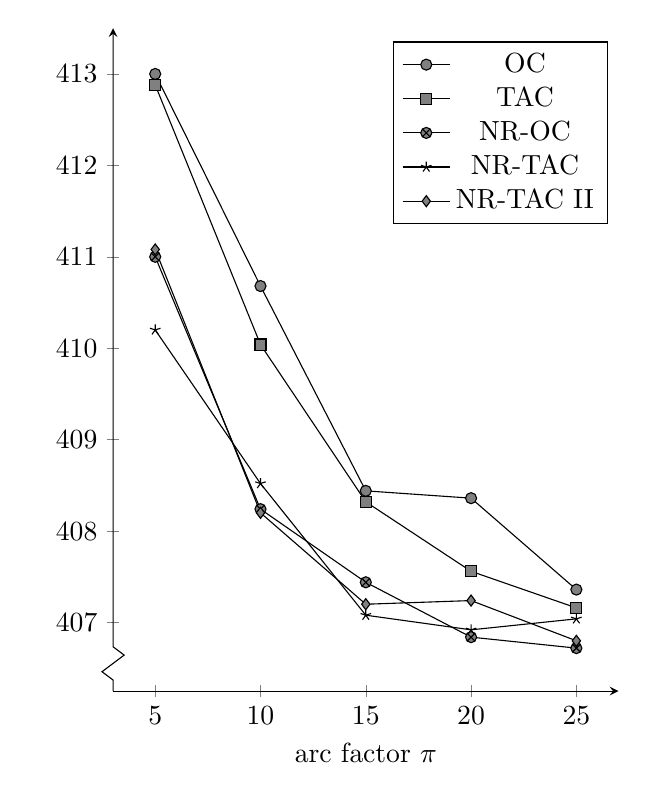
\begin{tikzpicture}
    \begin{axis}[
    	xlabel=arc factor $\pi$,
    	ylabel=\cnvavg,
		axis y discontinuity=crunch,
		axis x line=bottom,
		axis y line=left,
		ymin=406.25,
		ymax=413.5,
		xmin=3,
		xmax=27,
		cycle list name=black white,
		height=10cm,
		width=8cm
    ]
    \addplot coordinates {
		(5,413)
		(10,410.68)
		(15,408.44)
		(20,408.36)
		(25,407.36)
    };
    \addplot coordinates {
		(5,412.88)
		(10,410.04)
		(15,408.32)
		(20,407.56)
		(25,407.16)
    };
    \addplot coordinates {
		(5,411)
		(10,408.24)
		(15,407.44)
		(20,406.84)
		(25,406.72)
    };
    \addplot coordinates {
		(5,410.2)
		(10,408.52)
		(15,407.08)
		(20,406.92)
		(25,407.04)
    };
    \addplot coordinates {
        	(5,411.08)
        	(10,408.2)
        	(15,407.2)
        	(20,407.24)
        	(25,406.8)
    };
    \legend{OC,TAC,NR-OC,NR-TAC,NR-TAC II}
    \end{axis}
    \end{tikzpicture}
    
	\label{average}
} \hspace{0.8cm}
\subfigure[average run-time]{
    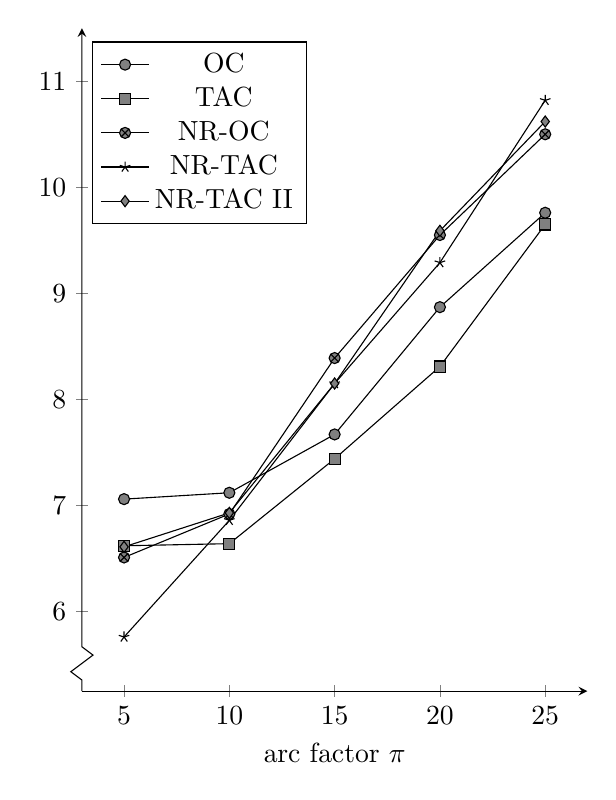
\begin{tikzpicture}
    \begin{axis}[
    	ylabel shift=-0.22cm,
    	xlabel=arc factor $\pi$,
    	ylabel=\cpu,
		axis y discontinuity=crunch,
		axis x line=bottom,
		axis y line=left,
		ymin=5.25,
		ymax=11.5,
		xmin=3,
		xmax=27,
		cycle list name=black white,
		height=10cm,
		width=8cm,
		legend style={at={(0.02, 0.98)}, anchor=north west}
    ]
    \addplot coordinates {
    	(5,7.06)
    	(10,7.12)
    	(15,7.67)
    	(20,8.87)
    	(25,9.76)
    };
    \addplot coordinates {
    	(5,6.62)
    	(10,6.64)
    	(15,7.44)
    	(20,8.31)
    	(25,9.65)
    };
    \addplot coordinates {
    	(5,6.51)
    	(10,6.92)
    	(15,8.39)
    	(20,9.55)
    	(25,10.5)
    };
    \addplot coordinates {
    	(5,5.76)
    	(10,6.86)
    	(15,8.15)
    	(20,9.29)
    	(25,10.82)
    };
    \addplot coordinates {
    	(5,6.61)
    	(10,6.93)
    	(15,8.15)
    	(20,9.59)
    	(25,10.62)
    };
    \legend{OC,TAC,NR-OC,NR-TAC,NR-TAC II}
    \end{axis}
    \end{tikzpicture}
	
	\label{times}
}
\label{both}
\caption{Illustration of the performance of \tsnew using the given combinations of \smslong and \sfaslong \added{and using the hierarchical objective}.}
\end{figure}

The results show that all \reducedcostbased \sms (\nrcs, \nrtacs, \nrtwotacs) exhibit a very similar behavior concerning the average \cnvs and run-time. The only exception are the results obtained with an \sfa of $\pi=5$: Here, the results of \nrtacs are notably superior to the other methods in terms of both solution quality and run-time, indicating that using this \sm seems reasonable when working with very small \reduced arc sets. 


The \reducedcostbased \sms are superior to the \standardSMS \sms (\costs, \tacs) in terms of solution quality and exhibit smaller run-times for an \sfa of $\pi=5$, similar run-times for $\pi=10$ and higher run-times for $\pi=15$ or above. Because no network relaxations must be solved for the \standardSMS \sms, one would expect consistently lower run-times for \costs and \tacs. The comparably high run-times of the \standardSMS \sms for small \sfas can be explained by an increased number of iterations caused by problems in finding high quality solutions. This is indicated by the inferior average \cnvs of the \standardSMS \sms for the small \sfas. Overall, it seems that the performance gains obtained by using \reducedcostbased \sms clearly outweigh the extra computational effort. Finally, we note that \tacs dominates \costs in terms of the average CNV and run-times. 

{Although the differences between the results obtained with the different \sms is often small, the Friedman test shows with high confidence that the choice of the \sm has a clear impact on the results. \added{In particular, we observed $p < 0.001$ for $\pi \leq 15$ and $p <0.05$ for larger $\pi$ values. Moreover,} the post-hoc analysis confirms with high confidence ($p < 0.001$ for $\pi=5$) that the results obtained with \reducedcostbased \sms are significantly different and better than those of the \standardSMS \sms.} 

As mentioned in Section~\ref{sec:sparsification}, we also investigate the influence of dynamically adding the arcs of the current best-known solution (BKS) to the \reduced arc set. To this end, Table~\ref{table:appendix} compares for all combinations of \sms and \sfas, the results obtained with (Column \emph{\baseC}) and without this technique (Column \emph{no-BKS}). We find that including the BKS provides superior or identical solution quality for all but two of the considered combinations (exceptions are \nrtwotacs with $\pi=20,25$) without increasing run-times. The negative effect of not including the BKS is notably stronger for small \sfas. {For $\pi=5$, the statistical tests confirm the superiority of including the BKS with high confidence ($p \ll 0.001$ for all \sms but \nrtwotacs, for which $p<0.05$).} We keep this feature for all of the following experiments \added{when using the hierarchical objective}.

%%%%%%%%%%%%%%%%%%%%%%%%%%%%%%%%%%%%%%%%%%%%%%%%%%%
\begin{table}[htbp]
\centering
\ra{1.2}
\scriptsize
\setlength{\tabcolsep}{3pt}
\begin{tabular}{@{}llrrcrrcrrcrrcrr@{}}
\toprule
\sfa & & \multicolumn{2}{c}{\textbf{\costs}} & & \multicolumn{2}{c}{\textbf{\tacs}}  & &  \multicolumn{2}{c}{\textbf{\nrcs}} & & \multicolumn{2}{c}{\textbf{\nrtacs}} & & \multicolumn{2}{c}{\textbf{\nrtwotacs}} \\
\cmidrule(lr){3-4} \cmidrule(lr){6-7} \cmidrule(lr){9-10} \cmidrule(lr){12-13}  \cmidrule(lr){15-16}   
 & & \emph{\baseC} & \emph{no-BKS} & &  \emph{\baseC} & \emph{no-BKS} & &  \emph{\baseC} & \emph{no-BKS} & &  \emph{\baseC} & \emph{no-BKS} & &  \emph{\baseC} & \emph{no-BKS} \\
\midrule
\multirow{2}{*}{$\mathbf{\boldsymbol{\pi}=5}$} 
& \cnvavg & 413.00 & 417.08 && 412.88 & 416.52 && 411.00 & 412.16 && 410.20 & 411.40 && 411.08 & 412.08 \\
& \cpu & 7.06 & 8.02 && 6.62 & 7.60 && 6.51 & 6.61 && 5.76 & 6.12 && 6.61 & 6.42  \\
\addlinespace
\multirow{2}{*}{$\mathbf{\boldsymbol{\pi}=10}$} 
& \cnvavg & 410.68 & 411.56 && 410.04 & 410.68 && 408.24 & 408.80 && 408.52 & 408.64 && 408.20 & 408.32 \\
& \cpu & 7.12 & 7.47 && 6.64 & 6.88 && 6.92 & 7.01 && 6.86 & 7.10 && 6.93 & 6.82 \\
\addlinespace
\multirow{2}{*}{$\mathbf{\boldsymbol{\pi}=15}$} 
& \cnvavg & 408.44 & 409.04 && 408.32 & 408.68 && 407.44 & 407.84 && 407.08 & 407.40 && 407.20 & 407.40  \\
& \cpu & 7.67 & 7.75 && 7.44 & 7.25 && 8.39 & 8.15 && 8.15 & 8.16 && 8.15 & 8.33 \\
\addlinespace
\multirow{2}{*}{$\mathbf{\boldsymbol{\pi}=20}$} 
& \cnvavg & 408.36 & 408.36 && 407.56 & 408.48 && 406.84 & 407.36 && 406.92 & 407.24 && 407.24 & 407.08 \\
& \cpu & 8.87 & 9.03 && 8.31 & 8.79 && 9.55 & 9.87 && 9.29 & 9.77 && 9.59 & 9.64\\
\addlinespace
\multirow{2}{*}{$\mathbf{\boldsymbol{\pi}=25}$} 
& \cnvavg & 407.36 & 408.04 && 407.16 & 407.72 && 406.72 & 406.72 && 407.04 & 407.28 && 406.80 & 406.40  \\
& \cpu & 9.76 & 10.34 && 9.65 & 9.51 && 10.50 & 10.42 && 10.82 & 10.98 && 10.62 & 10.57 \\
\bottomrule
\end{tabular}
\caption{Comparison of the performance of \tsnew not using the technique of including the arcs of the current best solution (denoted as \emph{no-BKS}) to the results obtained using the \base setting that uses this technique \added{when following the hierarchical objective}.}
\label{table:appendix}
\end{table}
%%%%%%%%%%%%%%%%%%%%%%%%%%%%%%%%%%%%%%%%%%%%%%%%%%%


\paragraph*{\added{Classical objective}} \added{Analogous to Table~\ref{table:appendix}, Table~\ref{distance:table1} reports the solution quality and run-time of the different \sms using the standard setting and the setting without dynamically adding the arcs of the best-known solution for the classical objective of minimizing the traveled distance.} 

\begin{table}[htbp]
\centering
\ra{1.2}
\scriptsize
\setlength{\tabcolsep}{3pt}
\begin{tabular}{@{}llrrcrrcrrcrrcrr@{}}
\toprule
\sfa & & \multicolumn{2}{c}{\textbf{\costs}} & & \multicolumn{2}{c}{\textbf{\tacs}}  & &  \multicolumn{2}{c}{\textbf{\nrcs}} & & \multicolumn{2}{c}{\textbf{\nrtacs}} & & \multicolumn{2}{c}{\textbf{\nrtwotacs}} \\
\cmidrule(lr){3-4} \cmidrule(lr){6-7} \cmidrule(lr){9-10} \cmidrule(lr){12-13}  \cmidrule(lr){15-16}   
 & & \emph{\baseC} & \emph{no-BKS} & &  \emph{\baseC} & \emph{no-BKS} & &  \emph{\baseC} & \emph{no-BKS} & &  \emph{\baseC} & \emph{no-BKS} & &  \emph{\baseC} & \emph{no-BKS} \\
\midrule
\multirow{2}{*}{$\mathbf{\boldsymbol{\pi}=5}$} 
& \ctdavg & 56\,335 & 56\,652 && 56\,259 & 56\,555 && 55\,441 & 55\,487 && 55\,374 & 55\,419 && 55\,358  & 55\,413 \\
 & \cpu & 6.18 & 5.87 && 6.30 & 6.04 && 6.78 & 6.28 && 6.65 & 6.29 && 6.78 & 6.60  \\
\addlinespace
\multirow{2}{*}{$\mathbf{\boldsymbol{\pi}=10}$} 
& \ctdavg &55\,387 & 55\,440 && 55\,390 & 55\,417 && 55\,018 & 55\,022 && 55\,024 & 55\,017 && 54\,992 & 55\,019 \\
 & \cpu & 7.22 & 7.32 && 7.31 &  6.93 &&  8.62 & 8.38 && 8.05 & 8.36 && 8.39 &8.24 \\
\addlinespace
\multirow{2}{*}{$\mathbf{\boldsymbol{\pi}=15}$} 
& \ctdavg & 55\,204 &  55\,212 && 55\,204 & 55\,196 && 54\,931 & 54\,940 && 54\,947 & 54\,939 && 54\,948 & 54\,935 \\
 & \cpu & 8.32 & 8.16 && 7.96  & 7.81 && 10.24 & 10.24  && 9.64 & 9.57 && 10.03 & 10.37 \\
\addlinespace
\multirow{2}{*}{$\mathbf{\boldsymbol{\pi}=20}$} 
& \ctdavg & 55\,061 & 55\,053 && 55\,057 & 55\,052 && 54\,912 & 54\,907 && 54\,932 & 54\,934 && 54\,912 & 54\,927 \\
 & \cpu & 9.46 & 9.68 && 9.39 & 9.24 && 11.57 & 11.63 &&  11.53 & 10.85 && 12.26 & 11.45 \\
\addlinespace
\multirow{2}{*}{$\mathbf{\boldsymbol{\pi}=25}$} 
& \ctdavg & 54\,999 & 55\,017 && 55\,016  & 55\,018 && 54\,925 & 54\,918 && 54\,912 & 54\,930 && 54\,930 & 54\,925 \\
 & \cpu & 10.88 & 10.68 && 10.29 & 10.05 && 12.67 & 12.62 && 12.24 & 12.33 && 13.03 & 13.03 \\
\bottomrule
\end{tabular}
\caption{\added{Comparison of the performance of \tsnew not using the technique of including the arcs of the current best solution (denoted as \emph{no-BKS}) to the results obtained using the \base setting that uses this technique when following the classical objective.}}
\label{distance:table1}
\end{table}

\added{We observe that the \standardSMS \sms \costs and \tacs show a very similar performance for the classical objective, except for $\pi=5$, for which \tacs provides a clearly better solution quality than \costs. However, both \standardSMS \sms are clearly inferior compared to the \reducedcostbased \sms with regard to solution quality, while requiring  lower run-times. The difference in run-times becomes larger for higher arc factors. This is confirmed by the statistical analysis that shows, with high confidence ($p < 0.05$ for $\pi \leq 15$), that the choice of the \sms has a strong impact on the quality of the results, whereas for $\pi\geq 20$ the choice of the \sms becomes less critical. The performance of all three \reducedcostbased \sms is relatively similar with a slight advantage for \nrtwotacs for the smallest arc factors $\pi=5,10$. Dynamically adding the arcs of the BKS on average slightly increases the run-time, while improving the solution quality for 16 out of the 25 tested combinations. The positive effect on solution quality is strongest for small \sfas: for $\pi=5$, the solution quality improves for all 5 \sms, for $\pi=10$ for 4 out of 5 \sms. The statistical analysis confirms the superiority of including the BKS with very high confidence, therefore, we also include this feature  for all the following experiments when using the classical objective.
}

%%%%%%%%%%%%%%%%%%%%%%%%%%%%%%%%%%%%%%%%%%%%%%%%%%%

\paragraph*{\added{Similarity of \sms and final selection of \sms to investigate}}

Besides the performance of the \sms, we are also interested in how different the \reduced arc sets generated by the \sms are. Table~\ref{table:overlap} shows for each pair of \sms the percentage of identically selected customer arcs for the \sfas $\pi=5, \pi=15$ and $\pi=25$. Note that in the computation of this percentage, we do not consider depot arcs or any dynamically added arcs in the \reduced arc set. 

\begin{table}[htbp]
\centering
\ra{1.2}
\scriptsize
\setlength{\tabcolsep}{5pt}
\begin{tabular}{@{}llrrrr@{}}
\toprule
\sms & \sfa  & \textbf{\tacs} & \textbf{\nrcs} & \textbf{\nrtacs} & \textbf{\nrtwotacs}\\
\midrule
\multirow{3}{*}{\textbf{\costs}}
& $\pi=5$ &    73.09\% &   73.30\% &  57.36\% & 68.71\% \\ 
& $\pi=15$ &   72.05\% & 85.04\% & 64.95\% & 78.17\% \\
& $\pi=25$ &  74.37\% & 89.85\% & 69.84\% & 84.29\% \\ 
\addlinespace
\multirow{3}{*}{\textbf{\tacs}} 
& $\pi=5$  &  \multicolumn{1}{c}{-} & 58.36\% & 73.27\% & 56.27\% \\
& $\pi=15$ &  \multicolumn{1}{c}{-} & 65.64\% & 85.57\%  & 61.96\%\\
& $\pi=25$ &  \multicolumn{1}{c}{-} & 70.08\% & 90.46\%  & 67.42\%\\ \\
\addlinespace
\multirow{3}{*}{\textbf{\nrcs}} 
& $\pi=5$ & \multicolumn{1}{c}{-} & \multicolumn{1}{c}{-} & 68.60\% & 79.79\% \\
& $\pi=15$ &  \multicolumn{1}{c}{-} &  \multicolumn{1}{c}{-} & 70.26\% & 82.53\%\\
& $\pi=25$  &  \multicolumn{1}{c}{-} &  \multicolumn{1}{c}{-} & 73.42\% & 86.84\%\\
\addlinespace
\multirow{3}{*}{\textbf{\nrtacs}} 
& $\pi=5$  & \multicolumn{1}{c}{-} & \multicolumn{1}{c}{-} &  \multicolumn{1}{c}{-} & 62.19\%\\
& $\pi=15$ &  \multicolumn{1}{c}{-} &  \multicolumn{1}{c}{-} &  \multicolumn{1}{c}{-} & 64.12\%\\
& $\pi=25$  &  \multicolumn{1}{c}{-} &  \multicolumn{1}{c}{-} &  \multicolumn{1}{c}{-} &68.86\%\\
\bottomrule
\end{tabular}
\caption{Overlap between the arcs selected by the different \smslong.}
\label{table:overlap}
\end{table}

We observe that the strongest overlap exists between the \standardSMS \sms and their reduced-cost counterpart (\costs/\nrcs and \tacs/\nrtacs), and between \nrcs and \nrtwotacs. Interestingly, the overlap strongly increases with the \sfa for some combinations (\costs/\nrcs, \costs/\nrtacs, \costs/\nrtwotacs, \tacs/\nrcs, \tacs/\nrtacs, \tacs/\nrtwotacs), while it remains relatively stable for the other combinations (\costs/\tacs, \nrcs/\nrtacs, \nrcs/\nrtwotacs, \nrtacs/\nrtwotacs).

Overall, we find that the arcs selected by different \sms differ significantly for many of the considered combinations, which renders the investigation of several \sms in the following studies reasonable. \added{However, to reduce the enormous computational effort of conducting the remaining experiments for all combinations of \sfas and \sms, we decided to:}
\begin{compactitem}
\item \added{remove \costs from the list of investigated \sms because}
\begin{inparaenum}[(i)] 
\item \added{for the hierarchical objective, it is dominated by \tacs with regard to both the average solution quality and the run-time, and}  
\item \added{for the classical objective, it shows a very similar performance to \tacs;} 
\end{inparaenum}
\item \added{keep \tacs in the following studies to avoid missing effects that may be caused by differences between \standardSMS and \reducedcostbased \sms;}
\item \added{exclude the \reducedcostbased \sm \nrtwotacs because} 
\begin{inparaenum}[(i)] 
\item \added{its idea is very similar to that of \nrtacs,} 
\item \added{the overlap between the arcs selected by this method and by \nrcs are rather high and also relatively constant for different \sfas, and} 
\item \added{for the hierarchical objective, \nrtacs shows clearly superior solution quality compared to \nrtwotacs for $\pi=5$, while, for the classical objective, results of \nrtwotacs and \nrtacs are more similar for $\pi=5$ (with only a slight advantage for \nrtwotacs).}
\end{inparaenum}
\end{compactitem}
Thus, the following experiments only investigate the \sms \tacs, \nrcs, and \nrtacs.  

\subsection{Incoming and Outgoing Generator Arcs for each Vertex}
\label{sec:52}
If instances contain geographical clusters of customers or isolated customers, it may happen that for some vertices the utilized \sm selects only very few incoming or outgoing arcs into the \reduced arc set. In this experiment, we investigate the impact of guaranteeing a minimum number of incoming and outgoing arcs for each customer vertex. Depot arcs are not counted. To this end, we check for each vertex $i$ whether the \reduced arc set contains at least $\minArcs = \lceil \frac{\pi \cdot (\maxCustomerSet + \vehicleNumber)}{4 \maxCustomerSet} \rceil$ incoming and also outgoing arcs. This number corresponds to half of the incoming/outgoing arcs of a customer if the arcs in the \reduced arc set were uniformly distributed among customers. If less than $\minArcs$ incoming/outgoing arcs exist, we additionally insert arcs according to the respective \sm until $|\delta^+(i)| = |\delta^-(i)| = \minArcs$, where $\delta^+(i)$ and $\delta^-(i)$ denote the forward and backward star of vertex $i$.  Table~\ref{table3} shows the results for different \sms and \sfas \added{for the hierarchical objective, Table~\ref{distance:table3} for the classical objective.} 

\begin{table}[htbp]
\centering
\ra{1.2}
\scriptsize
\setlength{\tabcolsep}{5pt}
\begin{tabular}{@{}llrrcrrcrr@{}}
\toprule
& & \multicolumn{2}{c}{\textbf{\tacs}} && \multicolumn{2}{c}{\textbf{\nrcs}} && \multicolumn{2}{c}{\textbf{\nrtacs}} \\
\cmidrule(lr){3-4} \cmidrule(lr){6-7} \cmidrule(lr){9-10}
\sfa  & & \emph{\baseC} & \emph{arcs added} && \emph{\baseC} & \emph{arcs added} && \emph{\baseC} & \emph{arcs added} \\
\midrule
\multirow{2}{*}{$\mathbf{\boldsymbol{\pi}=5}$} 
& \cnvavg & 412.88 & 411.76 && 411.00 & 410.64 && 410.20 & 410.20 \\% 411.08 & 410.52 \\
& \cpu & 6.62 & 6.19 && 6.51 & 6.17 && 5.76 & 5.95 \\ % 6.61 & 6.26 \\
\addlinespace
\multirow{2}{*}{$\mathbf{\boldsymbol{\pi}=10}$} 
& \cnvavg & 410.04 & 410.00 && 408.24 & 408.40 && 408.52 & 408.00 \\ % 408.20 & 408.48 \\
& \cpu & 6.64 & 6.56 && 6.92 & 7.11 && 6.86 & 7.06 \\ % 6.93 & 7.06 \\
\addlinespace
\multirow{2}{*}{$\mathbf{\boldsymbol{\pi}=15}$} 
& \cnvavg &408.32 & 408.80 && 407.44 & 407.40 && 407.08 & 407.32 \\ % 407.2 & 407.52 \\
& \cpu & 7.44 & 7.62 && 8.39 & 8.36 && 8.15 & 8.28 \\% 8.15 & 8.48 \\
\addlinespace
\multirow{2}{*}{$\mathbf{\boldsymbol{\pi}=20}$} 
& \cnvavg & 407.56 & 407.96 && 406.84 & 407.52 && 406.92 & 406.96 \\% 407.24 & 407.2 \\
& \cpu & 8.31 & 8.61 && 9.55 & 9.76 && 9.29 & 9.70 \\ %& 9.59 & 9.72 \\
\addlinespace
\multirow{2}{*}{$\mathbf{\boldsymbol{\pi}=25}$} 
& \cnvavg & 407.16 & 407.40 && 406.72 & 406.96 && 407.04 & 406.84 \\% 406.80 & 406.88 \\
& \cpu & 9.65 & 9.71 && 10.50 & 11.10 && 10.82 & 10.60 \\% & 10.62 & 10.96 \\
\bottomrule
\end{tabular}
\caption{Comparison of the performance of \tsnew including a minimum number of in- and outgoing arcs in the \reduced arc set (denoted as \emph{arcs added}) to the results obtained using the \base setting that does not include this feature \added{when following the hierarchical objective.}}
\label{table3}
\end{table}


\begin{table}[htbp]
\centering
\ra{1.2}
\scriptsize
\setlength{\tabcolsep}{5pt}
\begin{tabular}{@{}llrrcrrcrr@{}}
\toprule
& & \multicolumn{2}{c}{\textbf{\tacs}} && \multicolumn{2}{c}{\textbf{\nrcs}} && \multicolumn{2}{c}{\textbf{\nrtacs}} \\
\cmidrule(lr){3-4} \cmidrule(lr){6-7} \cmidrule(lr){9-10}
\sfa  & & \emph{\baseC} & \emph{arcs added} && \emph{\baseC} & \emph{arcs added} && \emph{\baseC} & \emph{arcs added} \\
\midrule
\multirow{2}{*}{$\mathbf{\boldsymbol{\pi}=5}$} 
& \ctdavg & 56\,259 & 55\,488 && 55\,441 & 55\,247 && 55\,374 & 55\,209 \\
& \cpu & 6.30 & 6.43 && 6.78 & 6.92 && 6.65 & 6.99 \\
\addlinespace
\multirow{2}{*}{$\mathbf{\boldsymbol{\pi}=10}$} 
& \ctdavg & 55\,390 & 55\,201 && 55\,018 & 54\,968 && 55\,024 & 54\,968 \\
& \cpu & 7.31 & 7.14 && 8.62 & 8.66 && 8.05 & 8.67 \\
\addlinespace
\multirow{2}{*}{$\mathbf{\boldsymbol{\pi}=15}$} 
& \ctdavg & 55\,204 & 54\,996 && 54\,931 & 54\,917&& 54\,947 & 54\,919 \\
& \cpu & 7.96 & 8.38 && 10.24 & 10.46 & &9.64 & 10.39 \\
\addlinespace
\multirow{2}{*}{$\mathbf{\boldsymbol{\pi}=20}$} 
& \ctdavg & 55\,057 & 54\,964 && 54\,912 & 54\,913 && 54\,932 & 54\,912 \\
& \cpu & 9.39 & 9.3 && 11.57 & 11.75 && 11.53 & 11.72 \\
\addlinespace
\multirow{2}{*}{$\mathbf{\boldsymbol{\pi}=25}$} 
& \ctdavg & 55\,016 & 54\,939 && 54\,925 & 54\,905 && 54\,912 & 54\,917 \\
& \cpu & 10.29 & 10.79 && 12.67 & 13.34 && 12.24 & 13.14 \\
\bottomrule
\end{tabular}
\caption{\added{Comparison of the performance of \tsnew including a minimum number of in- and outgoing arcs in the \reduced arc set (denoted as \emph{arcs added}) to the results obtained using the \base setting that does not include this feature when following the classical objective.}}
\label{distance:table3}
\end{table}

\paragraph*{\added{Hierarchical objective}} \added{{For the smallest \sfa $\pi=5$, we witness with high confidence ($p <0.05$)} a clear positive effect on solution quality, in some cases even within reduced run-times. For larger \sfas, no clear tendency can be found with regard to average solution quality. However, with four slight improvements and eight slight deteriorations for the tested combinations, the feature seems only recommendable for small \reduced arc sets. This result is quite reasonable, showing that for larger \reduced arc sets enough in- and outgoing arcs {to minimize the number of vehicles} are already contained, and therefore increasing this number to $\minArcs$ (which becomes larger with growing \sfa) has no clear positive effect.} 

\paragraph*{\added{Classical objective}} 
\added{For the arc factors $\pi=5,10,15$, a positive effect on solution 
quality can be observed for all \sms, while, generally, the run-time slightly increases. The strongest positive effect is achieved for \tacs. 
For the arc factors $\pi=20,25$, including the additional arcs leads to improved solution quality in four out of six cases; for the two cases with negative effect, the deterioration is very small. Summing up, for the classical objective, adding additional arcs is recommendable for all arc factors, however, the strongest positive impact can be found for small ones. The results are confirmed by the statistical analysis with high confidence.} 

\subsection{Treatment of depot arcs}
\label{sec:53}
As described above, depot arcs can make up for a major part of the arcs contained in the \reduced arc set. By completely removing depot arcs, the size of the \reduced arc set (more precisely of the static part of the \reduced arc set) can be reduced from  $|\granularSetm| = 2 \cdot \maxCustomerSet \cdot \vehicleNumber + \pi \cdot (\maxCustomerSet+\vehicleNumber)$ to  $|\granularSetm^{\mathit{noDepotArcs}}| =  \pi \cdot (\maxCustomerSet+\vehicleNumber)$. However, as noted by \citet{toth:03}, depot arcs have to be treated in a special way in order to guarantee a  good solution quality. We study the performance of the following strategies for including depot arcs in the \reduced arc set:
\begin{itemize}
\item [\textbf{All depot arcs (AA)}:] This is the \base case as used for the tests above. All depot arcs are inserted into the \reduced arc set in addition to the customer arcs selected by the utilized \sm. 
\item [\textbf{Separate depot arcs (SA)}:] In addition to the customer arcs selected according to the \sm, we  insert the first $\pi \cdot 2 \cdot \vehicleNumber$ depot arcs according to the \sm. 
\item [\textbf{No separate depot arcs (NA)}:] No depot arcs are additionally inserted into the \reduced arc set, i.e., depot arcs are only included as generator arcs if they are among the $\pi \cdot (\maxCustomerSet+\vehicleNumber)$ arcs selected by the utilized \sm. 
\end{itemize}

\added{Table~\ref{table4} provides a comparison of the results obtained with the three described strategies for all combinations of the three remaining \sms and the different \sfas for the hierarchical objective. Table~\ref{distance:table4} does the same for the classical objective.}

\begin{table}[htbp]
\centering
\ra{1.2}
\scriptsize 
\setlength{\tabcolsep}{4.5pt}
\begin{tabular}{@{}llrrrcrrrcrrr@{}}
\toprule
& & \multicolumn{3}{c}{\textbf{\tacs}} & & \multicolumn{3}{c}{\textbf{\nrcs}} & & \multicolumn{3}{c}{\textbf{\nrtacs}}\\
\cmidrule(lr){3-5} \cmidrule(lr){7-9} \cmidrule(lr){11-13}
\sfa &  & \multicolumn{1}{c}{\textit{AA}} & \multicolumn{1}{c}{\textit{SA}} & \multicolumn{1}{c}{\textit{NA}} & &  \multicolumn{1}{c}{\textit{AA}} & \multicolumn{1}{c}{\textit{SA}} & \multicolumn{1}{c}{\textit{NA}} &  &  \multicolumn{1}{c}{\textit{AA}} & \multicolumn{1}{c}{\textit{SA}} & \multicolumn{1}{c}{\textit{NA}} \\
\midrule
\multirow{2}{*}{ $\mathbf{\boldsymbol{\pi}=5}$} 
& \cnvavg &  412.88 & 415.20  & 415.92 & & 411.00 & 411.84 & 413.36 && 410.20 & 410.84 & 412.00 \\  
& \cpu  &  6.62 & 3.00 & 2.73 && 6.51 & 2.79 & 2.70 && 5.76 & 2.48 & 2.46 \\
\addlinespace
\multirow{2}{*}{ $\mathbf{\boldsymbol{\pi}=10}$} 
& \cnvavg &   410.04 & 410.52 & 411.04 && 408.24 & 408.96 & 409.68 && 408.52 & 408.32 & 409.76 \\
& \cpu  & 6.64 & 4.02 & 3.60 && 6.92 & 4.43 & 4.14 && 6.86 & 4.44 & 4.11 \\
\addlinespace
\multirow{2}{*}{ $\mathbf{\boldsymbol{\pi}=15}$} 
& \cnvavg &  408.32 & 408.76 & 409.24 && 407.44 & 407.60 & 408.48 && 407.08 & 407.48 & 408.04 \\ 
& \cpu  & 7.44 & 5.47 & 4.99 && 8.39 & 6.18  & 5.85 && 8.15 & 5.81  & 5.63 \\
\addlinespace
\multirow{2}{*}{ $\mathbf{\boldsymbol{\pi}=20}$} 
& \cnvavg &  407.56 & 408.04 & 407.88 && 406.84 & 407.08  & 408.00 && 406.92 & 407.40  & 407.48 \\
& \cpu  & 8.31 & 7.13 & 6.40 && 9.55 & 7.66  & 7.50 && 9.29 & 8.03 & 6.92 \\
\addlinespace
\multirow{2}{*}{ $\mathbf{\boldsymbol{\pi}=25}$} 
& \cnvavg &  407.16 & 407.60 & 407.68 && 406.72 & 406.80 & 407.32 && 407.04 & 406.96 & 406.92 \\
& \cpu  & 9.65 & 8.60 & 7.81 && 10.50 & 9.49 & 8.89 && 10.82 & 8.91 & 8.07 \\
\bottomrule
\end{tabular}
\caption{Comparison of the performance of \tsnew \added{for the hierarchical objective} using the different strategies AA, SA, and NA for including depot arcs into the \reduced arc set.}
\label{table4}
\end{table}

\begin{table}[htbp]
\centering
\ra{1.2}
\scriptsize 
\setlength{\tabcolsep}{4.5pt}
\begin{tabular}{@{}llrrrcrrrcrrr@{}}
\toprule
& & \multicolumn{3}{c}{\textbf{\tacs}} & & \multicolumn{3}{c}{\textbf{\nrcs}} & & \multicolumn{3}{c}{\textbf{\nrtacs}}\\
\cmidrule(lr){3-5} \cmidrule(lr){7-9} \cmidrule(lr){11-13}
\sfa &  & \multicolumn{1}{c}{\textit{AA}} & \multicolumn{1}{c}{\textit{SA}} & \multicolumn{1}{c}{\textit{NA}} & &  \multicolumn{1}{c}{\textit{AA}} & \multicolumn{1}{c}{\textit{SA}} & \multicolumn{1}{c}{\textit{NA}} &  &  \multicolumn{1}{c}{\textit{AA}} & \multicolumn{1}{c}{\textit{SA}} & \multicolumn{1}{c}{\textit{NA}} \\
\midrule
\multirow{2}{*}{ $\mathbf{\boldsymbol{\pi}=5}$} 
& \ctdavg & 56\,259 & 57\,218 & 58\,299 && 55\,441 & 55\,529 & 55\,890 && 55\,374 & 55\,508 & 55\,812 \\
& \cpu  & 6.30 & 1.81 & 1.60 && 6.78 & 2.17 & 1.99 && 6.65 & 2.18 & 2.03 \\
\addlinespace
\multirow{2}{*}{ $\mathbf{\boldsymbol{\pi}=10}$} 
& \ctdavg &  55\,390 & 55\,518 & 55\,558 && 55\,018 & 55\,009 & 55\,181 && 55\,024 & 55\,010 & 55\,131 \\
& \cpu  & 7.31 & 3.26 & 2.91 && 8.62 & 4.38 & 3.92 && 8.05 & 4.15 & 3.78 \\
\addlinespace
\multirow{2}{*}{ $\mathbf{\boldsymbol{\pi}=15}$} 
& \ctdavg & 55\,204 & 55\,236 & 55\,250 && 54\,931 & 54\,930 & 55\,002 && 54\,947 & 54\,943 & 55\,026 \\
& \cpu  & 7.96 & 4.62 & 4.03 && 10.24 & 6.36 & 5.77& & 9.64 & 6.11 & 5.60  \\
\addlinespace
\multirow{2}{*}{ $\mathbf{\boldsymbol{\pi}=20}$} 
& \ctdavg & 55\,057 & 55\,066 & 55\,100 && 54\,912 & 54\,917 & 54\,959 && 54\,932 & 54\,909 & 54\,967 \\
& \cpu  & 9.39 & 6.32 & 5.6 && 11.57 & 8.21 & 7.58 && 11.53 & 7.89 & 7.34 \\
\addlinespace
\multirow{2}{*}{ $\mathbf{\boldsymbol{\pi}=25}$} 
& \ctdavg & 55\,016 & 55\,023 & 55\,024 && 54\,925 & 54\,906 & 54\,920 && 54\,912 & 54\,921 & 54\,932 \\
& \cpu  & 10.29 & 7.72 & 6.77 && 12.67 & 9.63 & 9.09 && 12.24 & 9.43 & 8.56 \\
\bottomrule
\end{tabular}
\caption{\added{Comparison of the performance of \tsnew for the classical objective using the different strategies AA, SA, and NA for including depot arcs into the \reduced arc set.}}
\label{distance:table4}
\end{table}

\paragraph*{\added{Hierarchical objective}}
\added{For $13$ out of the $15$ tested combinations, the best solution quality is obtained using the AA strategy. NA achieves the fastest run-time of all strategies for all tested combinations. The difference in solution quality and run-time between the two extreme strategies, i.e., AA and NA, is highest and statistically significant for $\pi=5$ and gradually reduces for higher \sfas. Run-times for the intermediate strategy SA are relatively close to those of NA and its solution quality generally lies between that of AA and NA. }

\paragraph*{\added{Classical objective}} \added{NA shows the lowest run-time for all tested combinations, and SA requires only slightly more time. The run-time difference compared to strategy AA is strongest for $\pi=5$ with a factor of $>3$ and decreases with higher arc factors (to a factor of roughly 1.5 for $\pi=25$). Strategy AA achieves the best solution quality for 9 out of 15 combinations, especially for all combinations with $\pi=5$ and all combinations using the \sm \tacs. For many combinations, SA shows a very good tradeoff between solution quality (with the best quality for 6 out of 15 combinations and results close to those of AA for many other combinations especially those with the \reducedcostbased \sms)  and run-time. This is confirmed with high confidence ($p<0.001$) by the statistical analysis. } 

\paragraph{\added{Recommendations}}
\added{If the main focus is on solution quality, the AA strategy seems {preferable}. This is especially true for a small \sfa of $\pi=5$, for which the performance differences between the two extreme strategies are high. If the focus is more on run-time, using the SA strategy seems reasonable as a good trade-off between solution quality and run-time is achieved for the large majority of tested combinations.}

\subsection{Dynamic Sparsification}
\label{sec:54}
As proposed by \citet{toth:03}, dynamically adjusting the size of the \reduced arc set can be used to diversify (by doing weaker sparsification) and intensify (by doing stronger sparsification) the search. Therefore, we implement the following dynamic sparsification procedure to investigate the effect of dynamic sparsification on the performance of \tsnew:
\begin{enumerate}
\item We start with a base \sfa $\pi_{\mathit{base}}$ and compare solutions after every $\theta=100$ iterations. 
\item After every $\theta$ iterations in which no improvement has taken place, a diversification phase with $\pi = 2 \cdot \pi_{\mathit{base}}$ is started and lasts for $\theta$ iterations. 
\item \added{When following the hierarchical objective}, as long as no feasible solution has been found with the given number of vehicles, the base \sfa is increased to $\pi_{\mathit{base}}=  1.5 \cdot \pi_{\mathit{base}}$ every
    $\gamma=1000$ iterations. After a feasible solution has been found, the base \sfa is reset to its original value. 
 \end{enumerate}

\added{Tables~\ref{table45} (hierarchical objective) and \ref{distance:table45} (classical objective)} show the comparison of the results obtained with dynamic sparsification for $\pi_{\mathit{base}} = 2.5,  5, 10,15$ compared to those obtained when statically using the corresponding \sfa. Note that we refrain from calculating the static results for an \sfa of $\pi=2.5$ because this \sfa is simply too small to achieve meaningful results when used in a static context.  

\begin{table}[htbp]
\centering
\ra{1.2}
\scriptsize
\setlength{\tabcolsep}{5pt}
\begin{tabular}{@{}llcrrcrrcrr@{}}
\toprule
& && \multicolumn{2}{c}{\textbf{\tacs}} && \multicolumn{2}{c}{\textbf{\nrcs}} && \multicolumn{2}{c}{\textbf{\nrtacs}}\\
\cmidrule(lr){4-5} \cmidrule(lr){7-8} \cmidrule(lr){10-11}
 (base) \sfa & & & \emph{static} & \emph{dynamic} & &  \emph{static} & \emph{dynamic} & & \emph{static} & \emph{dynamic}  \\
\midrule
\multirow{2}{*}{ $\mathbf{\boldsymbol{\pi}=2.5}$} 
 & \cnvavg &&  \multicolumn{1}{c}{-} & 406.76 && \multicolumn{1}{c}{-}   &  406.80  && \multicolumn{1}{c}{-}  &  406.52 \\ 		
& \cpu &&  \multicolumn{1}{c}{-}  & 8.64 && \multicolumn{1}{c}{-}  & 9.09 && \multicolumn{1}{c}{-}  & 8.65 \\ 
\addlinespace
\multirow{2}{*}{ $\mathbf{\boldsymbol{\pi}=5}$} 
& \cnvavg && 412.88 & 406.76 && 411.00 & 406.32 && 410.20 & 406.24 \\
& \cpu && 6.62 & 9.21 && 6.51 & 9.63 && 5.76 & 9.15 \\ 
\addlinespace
\multirow{2}{*}{ $\mathbf{\boldsymbol{\pi}=10}$} 
& \cnvavg &&  410.04 & 406.68 & & 408.24 & 406.60 && 408.52 & 406.52 \\ 
& \cpu && 6.64 & 10.97 && 6.92 & 11.31 && 6.86 & 12.23 \\
\addlinespace
\multirow{2}{*}{ $\mathbf{\boldsymbol{\pi}=15}$} 
& \cnvavg &&  408.32 & 406.36 && 407.44 & 407.20 && 407.08 & 406.24 \\ 
& \cpu & & 7.44 & 12.47 & & 8.39 & 14.23 & & 8.15 & 13.03 \\ 
\bottomrule
\end{tabular}
\caption{Performance comparison of \tsnew using static and dynamic sparsification \added{when following the hierarchical objective}.}
\label{table45}
\end{table}

\begin{table}[htbp]
\centering
\ra{1.2}
\scriptsize
\setlength{\tabcolsep}{5pt}
\begin{tabular}{@{}llcrrcrrcrr@{}}
\toprule
& && \multicolumn{2}{c}{\textbf{\tacs}} && \multicolumn{2}{c}{\textbf{\nrcs}} && \multicolumn{2}{c}{\textbf{\nrtacs}}\\
\cmidrule(lr){4-5} \cmidrule(lr){7-8} \cmidrule(lr){10-11}
 (base) \sfa & & & \emph{static} & \emph{dynamic} & &  \emph{static} & \emph{dynamic} & & \emph{static} & \emph{dynamic}  \\
\midrule
\multirow{2}{*}{ $\mathbf{\boldsymbol{\pi}=2.5}$} 
 & \ctdavg &&  \multicolumn{1}{c}{-} & 56\,487  && \multicolumn{1}{c}{-}   &  55\,541 && \multicolumn{1}{c}{-}  &  55\,419 \\
& \cpu &&  \multicolumn{1}{c}{-}  & 6.64  && \multicolumn{1}{c}{-}  & 6.78  &&  \multicolumn{1}{c}{-}  & 7.10 \\ 
\addlinespace
\multirow{2}{*}{ $\mathbf{\boldsymbol{\pi}=5}$} 
& \ctdavg && 56\,259 & 55\,474 && 55\,441 & 55\,060 && 55\,374 & 55\,041 \\
& \cpu && 6.30 & 7.99 && 6.78 & 8.46 && 6.65 & 8.89 \\
\addlinespace
\multirow{2}{*}{ $\mathbf{\boldsymbol{\pi}=10}$} 
&\ctdavg && 55\,390 & 55\,099 && 55\,018 & 54\,918 && 55\,024 & 54\,917 \\
& \cpu && 7.31 & 10.25 && 8.62 & 12.49 && 8.05 & 11.77 \\
\addlinespace
\multirow{2}{*}{ $\mathbf{\boldsymbol{\pi}=15}$} 
& \ctdavg && 55\,204 & 54\,989 && 54\,931 & 54\,887 && 54\,947 & 54\,916 \\
& \cpu && 7.96 & 12.30 && 10.24 & 14.24 && 9.64 & 14.59 \\
\bottomrule
\end{tabular}
\caption{\added{Performance comparison of \tsnew using static and dynamic sparsification when following the classical objective.}}
\label{distance:table45}
\end{table}

\paragraph*{\added{Hierarchical objective}}
\added{For all \sms, dynamic sparsification yields, with high confidence ($p \ll 0.001$), significantly improved solution quality compared to the static variant, however, the dynamic variant takes longer when using the corresponding \sfa as base. The results of the dynamic sparsification are rather robust concerning the base \sfa used, which recommends to use a very small base \sfa as this leads to reduced run-times. Finally, it should be noted that dynamic sparsification also works very good with the \standardSMS \sm \tacs and the difference to the {\reducedcostbased} \sms is quite small.}

\paragraph*{\added{Classical objective}} \added{For all tested combinations, the results achieved with dynamic sparsification show, with high confidence $(p \ll 0.001)$, better solution quality but higher run-times than the static results. Contrary to the tests with the hierarchical objective, increasing the base \sfa leads to both clearly improved solution quality and higher run-times. A good tradeoff between quality and run-time is found for $\pi=5$.} 


\paragraph*{\added{Parameter setting for dynamic sparsification}}
\added{The results above are clearly also dependent on the values of the parameters $\theta$ and $\gamma$ of our dynamic sparsification technique. To validate that the setting $\theta=100$ and $\gamma=1000$ achieves reasonable results, we conduct a parameter study (see Table~\ref{tab:param:dyn:hier}) in which we compare the results of the combinations $\theta=\{50, 100, 150\}; \gamma=\theta \cdot \{5,10,15\}$ for the hierarchical objective using  the \sm \nrtacs with $\pi_{\mathit{base}}=2.5$. For the classical objective, we test the values   $\theta=\{50, 100, 150\}$ using  the \sm \nrtacs with $\pi_{\mathit{base}}=5$. The results show that our sparsification technique is very robust with regard to changes of its parameters and that the original setting ($\theta=100, \gamma=1000$) achieves a very good tradeoff between solution quality and run-times.}

\begin{table}[htbp]
\centering
\ra{1.2}
\scriptsize
\setlength{\tabcolsep}{5pt}
\begin{tabular}{@{}clcrcrcr@{}}
\toprule
$\mathbf{\boldsymbol{\theta}}$ & && \multicolumn{1}{c}{\textbf{50}} && \multicolumn{1}{c}{\textbf{100}} && \multicolumn{1}{c}{\textbf{150}}\\
\midrule
\multicolumn{2}{l}{\textbf{Hierarchical objective}} \\
\multirow{2}{*}{$\mathbf{\boldsymbol{\gamma}=5 \cdot \boldsymbol{\theta} }$} 
 & \cnvavg && 406.60 && 406.60 && 406.84 \\		
& \cpu &&  10.29 && 9.32 && 9.46 \\
\addlinespace
\multirow{2}{*}{$\mathbf{\boldsymbol{\gamma}=10 \cdot \boldsymbol{\theta} }$} 
& \cnvavg && 	406.56 && 406.52	&& 406.56\\
& \cpu &&9.36 && 8.65 && 9.00 \\
\addlinespace
\multirow{2}{*}{$\mathbf{\boldsymbol{\gamma}=15 \cdot \boldsymbol{\theta} }$} 
& \cnvavg && 406.76 && 406.92	&& 407.08  \\ 
& \cpu &&  9.27 && 8.73 && 8.86\\
\addlinespace
\multicolumn{2}{l}{\textbf{Classical objective}} \\
& \ctdavg && 	55\,043 &&	55\,041  &&	55\,044\\
& \cpu && 8.93 &&	8.89 && 9.05 \\
\bottomrule
\end{tabular}
\caption{\added{Parameter setting for the dynamic sparsification.}}
\label{tab:param:dyn:hier}
\end{table}

\subsection{Advanced \smsHeading}
\label{sec:55}
In this section, we investigate the idea of combining the results obtained with the basic \sms described in Section~\ref{sec:sparsification} in order to obtain \sms of better quality. We study five advanced \sms that combine \tacs, \nrcs, and \nrtacs as follows (note that the number of arcs selected by the advanced \sm is given by the \sfa $\bar{\pi}$):
\begin{enumerate}
\item \textbf{Combined order}: We fill the \reduced arc set by taking the first element according to the order given by \sm \tacs, then the first of \sm \nrcs, and \nrtacs, then the second element of each \standalone \sm and so on until we have reached $\bar{\pi} \cdot (\maxCustomerSet + \vehicleNumber)$ elements.
\item \textbf{Union}: The \reduced arc set is constructed by  the union of the arc sets obtained with the \sms  \tacs, \nrcs, and \nrtacs, each using an \sfa of $\pi = \frac{2}{3} \bar{\pi}$. Note that this leads to a size of the \reduced arc set that is usually different from $\bar{\pi} \cdot (\maxCustomerSet + \vehicleNumber)$.
\item \textbf{Intersection}: The \reduced arc set is constructed by the intersection of the arc sets obtained with the \sms  \tacs, \nrcs, and \nrtacs, each using an \sfa of $\pi = \frac{4}{3} \bar{\pi}$. This also leads to a size of the \reduced arc set that is usually different from $\bar{\pi} \cdot (\maxCustomerSet + \vehicleNumber)$.
\item \textbf{Order by rank}: This \sm first determines the ranks of the arcs selected according to \tacs, \nrcs, and \nrtacs  using the \sfa $\pi = \bar{\pi}$, and subsequently 
for each arc its rank for the different \sms is summed up. Then, the elements are ordered according to nondecreasing values of the summed up ranks (breaking ties arbitrarily), and the first $\bar{\pi} \cdot (\maxCustomerSet + \vehicleNumber)$ elements are inserted into the \reduced arc set. 
\item \textbf{Order by  logarithmized rank}: This \sm is similar to the previous one, but here we sum up the logarithms of the ranks.
\end{enumerate}

\added{Tables~\ref{table7} and \ref{table7:classical} show the results of the described advanced \sms for the \sfas $\bar{\pi}=5,10,15,20,25$ for the hierarchical and the classical objective, respectively. For comparison reasons, the results of the two \standalone \sms \nrcs and \nrtacs for \sfa $\pi = \bar{\pi}$ are also given.} 

\begin{table}[htbp]
\centering
\ra{1.2}
\scriptsize
\setlength{\tabcolsep}{4.5pt}
\begin{tabular}{@{}llrrrrrrcrr@{}}
\toprule
\sfa & & \textbf{Comb.\,O.} & \textbf{Union} & \textbf{Intersection} & \textbf{O.\,Rank} & \textbf{O.\,Log.\,Rank} & & \textbf{\nrcs} & \textbf{\nrtacs} \\
\midrule
\multirow{2}{*}{ $\mathbf{\boldsymbol{\bar{\pi}}=5}$} 
& \cnvavg &  411.60 & 411.60 & 412.20 & 410.60 & 410.56 & & 411.00 & 410.20 \\  
& \cpu & 8.05 & 7.15 & 7.65  & 6.03 & 6.00 & &  6.51 & 5.76  \\
\addlinespace
\multirow{2}{*}{ $\mathbf{\boldsymbol{\bar{\pi}}=10}$}
& \cnvavg & 409.16 & 409.48 & 408.56 & 407.76 & 408.20 && 408.24 &  408.52 \\
& \cpu & 7.02 & 6.22 & 6.01 & 5.47 & 5.57 && 6.92   & 6.86 \\
\addlinespace
\multirow{2}{*}{ $\mathbf{\boldsymbol{\bar{\pi}}=15}$}
& \cnvavg &  407.96 & 407.92 & 408.32 & 407.88 & 407.88 & &  407.44 & 407.08 \\
& \cpu & 9.08 & 8.29 & 8.91 & 8.20 & 7.80 && 8.39 & 8.15 \\
\addlinespace
\multirow{2}{*}{ $\mathbf{\boldsymbol{\bar{\pi}}=20}$}
& \cnvavg & 407.56 & 407.44 & 407.36  & 407.72 & 407.40 &&406.84 & 406.92 \\
& \cpu & 8.95 & 7.89 & 8.01  & 7.89 & 7.51 &&9.55& 9.29 \\
\addlinespace
\multirow{2}{*}{ $\mathbf{\boldsymbol{\bar{\pi}}=25}$} 
& \cnvavg & 407.28 & 407.16 & 407.40 & 406.92 & 406.88 && 406.72 & 407.04  \\
& \cpu & 11.50 & 10.26 & 11.63 & 10.25 & 10.17 && 10.50 & 10.82  \\
\bottomrule
\end{tabular}
\caption{Results of the advanced \sms for the \sfas $\bar{\pi}=5,10,15,20,25$ in comparison to the results of the \standalone \sms \nrcs, and \nrtacs with $\pi = \bar{\pi}$ \added{when following the hierarchical objective.}}
\label{table7}
\end{table}

\begin{table}[htbp]
\centering
\ra{1.2}
\scriptsize
\setlength{\tabcolsep}{4.5pt}
\begin{tabular}{@{}llrrrrrrcrr@{}}
\toprule
\sfa & & \textbf{Comb.\,O.} & \textbf{Union} & \textbf{Intersection} & \textbf{O.\,Rank} & \textbf{O.\,Log.\,Rank} & & \textbf{\nrcs} & \textbf{\nrtacs} \\
\midrule
\multirow{2}{*}{ $\mathbf{\boldsymbol{\bar{\pi}}=5}$} 
& \cnvavg & 55\,559 & 55\,512 & 55\,825 & 55\,355 & 55\,351 &  & 55\,441 & 55\,374 \\
& \cpu & 8.85 & 7.27 & 7.25 & 6.81 & 6.60 &  & 6.78 & 6.65 \\
\addlinespace
\multirow{2}{*}{ $\mathbf{\boldsymbol{\bar{\pi}}=10}$}
& \cnvavg & 55\,088 & 55\,078 & 55\,276 & 54\,995 & 55\,016 &  & 55\,018 & 55\,024 \\
& \cpu &  10.20 & 8.65 & 8.41 & 8.25 & 7.98 &  & 8.62 & 8.05 \\
\addlinespace
\multirow{2}{*}{ $\mathbf{\boldsymbol{\bar{\pi}}=15}$}
& \cnvavg & 54\,963 & 54\,956 & 55\,060 & 54\,949 & 54\,962 &  & 54\,931 & 54\,947 \\
& \cpu &  11.71 & 10.44 & 9.78 & 9.84 & 9.09 &  & 10.24 & 9.64 \\
\addlinespace
\multirow{2}{*}{ $\mathbf{\boldsymbol{\bar{\pi}}=20}$}
& \cnvavg & 54\,917 & 54\,921 & 55\,000 & 54\,934 & 54\,928 &  & 54\,912 & 54\,932 \\
& \cpu & 13.34 & 11.78 & 11.07 & 10.76 & 10.63 &  & 11.57 & 11.53 \\
\addlinespace
\multirow{2}{*}{ $\mathbf{\boldsymbol{\bar{\pi}}=25}$} 
& \cnvavg & 54\,895 & 54\,898 & 54\,956 & 54\,920 & 54\,905 &  & 54\,925 & 54\,912 \\
& \cpu & 15.34 & 13.15 & 12.71 & 12.03 & 11.84 &  & 12.67 & 12.24 \\
\bottomrule
\end{tabular}
\caption{\added{Results of the advanced \sms for the \sfas $\bar{\pi}=5,10,15,20,25$ in comparison to the results of the \standalone \sms \nrcs, and \nrtacs with $\pi = \bar{\pi}$ when following the classical objective.}}
\label{table7:classical}
\end{table}

\paragraph*{\added{Hierarchical objective}}
\added{For all investigated \sfas, the best solution is either provided by one of the  \standalone or rank-based \sms, the methods \emph{Union}, \emph{Combined order}, and \emph{Intersection} are not able to match that quality. The \standalone \sms provide superior quality compared to the rank-based method for all \sfas but $\bar{\pi}=\pi=10$.}

\paragraph*{\added{Classical objective}}
\added{For all \sfas but $\bar{\pi}=\pi=25$, the best solution quality is again either provided by one of the  \standalone or rank-based \sms. The rank-based methods are slightly superior for the smaller \sfas, the \standalone \sms for the larger \sfas.} 

\paragraph{\added{Recommendations}}
Taking into account the additional implementation effort, the discussed results do not recommend the implementation of the advanced \sms. We can only speculate about the reasons for their lower-than-expected performance: although the arcs selected by the different \sms do differ (see Table~\ref{table:overlap}), it may be that the quality of the different arcs is rather similar, so that no real diversification can be achieved by the advanced \sms.

\subsection{Comparison to the state-of-the-art}
\label{sec:56}
\added{In the following, we compare the performance of \tsnew to that of our TS using complete neighborhoods, denoted as \tscomplete. For the hierarchical objective, we additionally compare \tsnew to the best-performing VRPTW metaheuristics from the literature; for the classical objective, we assess the solution quality of \tsnew by comparing to the optimal solutions found by exact methods. \tsnew aims at very fast run-times without compromising too much solution quality and therefore uses the following final configuration based on the insights gained from the previous experiments (only few differences are necessary based on the type of objective that we follow): We choose dynamic sparsification with a base \sfa of $\pi_{\mathit{base}}=2.5$  and \nrtacs as \sm for the hierarchical objective. For the classical objective, we use $\pi_{\mathit{base}}=5$ to achieve the best tradeoff between run-time and solution quality. To counteract the higher run-times caused by the dynamic sparsification, we restrict the increase of the base \sfa to a maximum value of $10$ for the hierarchical objective. Moreover, we apply the strategy SA for including depot arcs, and we guarantee a minimum number of incoming and outgoing arcs per vertex.}   

\paragraph*{\added{Hierarchical objective}}
In Table~\ref{ds:tab:compareVRPTW}, we present the results of \tsnew, and \tscomplete in comparison to the best-performing metaheuristics from the literature: \textbf{HY} \citep*{hashimoto:08:path}, \textbf{LCK} \citep*{bouthillier:05b}, \textbf{BVH} \citep*{bent:04}, \textbf{PGDR} \citep*{prescott:09}, \textbf{HYI} \citep*{hashimoto:08:iterated}, \textbf{LZ} \citep*{lim:07}, \textbf{PR} \citep*{pisinger:07}, \textbf{RTI} \citep*{repoussis:09}, \textbf{NBD} \citep*{nagata:10}, \textbf{B} \citep*{braysy:03}, and \textbf{VCGP} \citep*{vidal:13}. For each method, the solution quality in terms of vehicle number and traveled distance is reported. We follow the common procedure and give averages over the problem classes C, R, and RC, and the \cnvs, and the \ctds. 

\added{As described above, \tsnew does not take care of vehicle minimization but is started with the number of vehicles equal to the number of routes of the best-known solution reported in the literature. This approach is adopted by several authors in the literature \citep[see, e.g.,][]{hashimoto:08:path,hashimoto:08:iterated,cordeau:12}. We compare to the best methods from the literature, not differentiating between methods with vehicle minimization component and those without. We want to point out that the resulting comparison, although consistently performed by the research community, may be seen as not completely fair.}

To make the comparison of the run-times of the different methods as fair as possible, we follow the approach of \citet{gendreau:10:vrptw} and translate the different hardware used in the numerical experiments of the papers into a comparable time measure. \citet{gendreau:10:vrptw} derive a relative estimated speed compared to a Pentium 4 2,8 GHz processor for each of the used computers based on the performance indicators of \citet{dongarra:11}.  To translate into the common time measure, the relative speed factor is multiplied by the number of employed processors, the number of executed runs, and the run-time in minutes (see Table~\ref{ds:tab:compareVRPTW}). We use the reported values of \citet{gendreau:10:vrptw} and estimate the speed factor of our Intel Core i7 processor with 3.50 GHz in comparison to their Pentium 4 to a value of $2.60$, after running the LINPACK benchmark used in \citet{dongarra:11} on our machine. \added{Such techniques for comparing the run-times of different methods are clearly not exact because run-times also depend on the programming language used, the operating system and the installed memory}. Nevertheless, we hope to provide a good indication about the speed of the heuristics. 

%%%%%%%%%%%%%%%%%%%%%%%%%%%%%%%%%%%%%%%%%%%%%%%%%%%%%%%%%%%%%%%%%%%%%%%%%%%%%%%%%%%%%%%%%%%%%%%%%%%%%%%%%
\begin{sidewaystable}
\setlength{\tabcolsep}{4pt}
  \scriptsize
  \centering
\ra{1.2}
 \begin{tabular}{@{}lcrcrcrcrcrcrcrcrcrcrcrccrcr@{}}
\toprule
& & \multicolumn{1}{c}{\textbf{HY}} & & \multicolumn{1}{c}{\textbf{LCK}} & & \multicolumn{1}{c}{\textbf{BVH}} & & \multicolumn{1}{c}{\textbf{PGDR}} & & \multicolumn{1}{c}{\textbf{HYI}} & & \multicolumn{1}{c}{\textbf{LZ}} & & \multicolumn{1}{c}{\textbf{PR}} & & \multicolumn{1}{c}{\textbf{RTI}} & & \multicolumn{1}{c}{\textbf{NBD}} & & \multicolumn{1}{c}{\textbf{B}} & & \textbf{VCGP} & & & \multicolumn{1}{c}{\textbf{\tsnew}} && \multicolumn{1}{c}{\textbf{\tscomplete}} \\
\midrule
\textbf{R1} &  & 11.92 &  & 11.92 &  & 11.92 &  & \textbf{11.92} &  & 11.92 &  & 11.92 &  & 11.92 &  & 11.92 &  & \textbf{11.92} &  & 11.92 &  & 11.92 &  & &  11.92 &  & 11.92\\
 &  & 1216.70 &  & 1214.20 &  & 1213.25 &  & \textbf{1210.34} &  & 1213.18 &  & 1213.61 &  & 1212.39 &  & 1210.82 &  & \textbf{1210.34} &  & 1222.12 &  & 1210.69 &  & &  1229.43 & & 1220.83\\
\addlinespace
\textbf{R2} &  & 2.73 &  & 2.73 &  & 2.73 &  & 2.73 &  & 2.73 &  & 2.73 &  & 2.73 &  & 2.73 &  & \textbf{2.73} &  & 2.73 &  & 2.73 &  & & 2.73 &  & 2.73\\
 &  & 961.28 &  & 954.32 &  & 966.37 &  & 955.74 &  & 955.61 &  & 961.05 &  & 957.72 &  & 952.67 &  & \textbf{951.03} &  & 975.12 &  & 951.51 &  & & 974.59 & & 959.86 \\
\addlinespace
\textbf{C1} &  & \textbf{10.00} &  & \textbf{10.00} &  & \textbf{10.00} &  & \textbf{10.00} &  & \textbf{10.00} &  & \textbf{10.00} &  & \textbf{10.00} &  & \textbf{10.00} &  & \textbf{10.00} &  & \textbf{10.00} &  & \textbf{10.00} &  & & \textbf{10.00} &  & \textbf{10.00} \\
 &  & \textbf{828.38} &  & \textbf{828.38} &  & \textbf{828.38} &  & \textbf{828.38} &  & \textbf{828.38} &  & \textbf{828.38} &  & \textbf{828.38} &  & \textbf{828.38} &  & \textbf{828.38} &  & \textbf{828.38} &  & \textbf{828.38} &  & & \textbf{828.38} &  & \textbf{828.38} \\
\addlinespace
\textbf{C2} &  & \textbf{3.00} &  & \textbf{3.00} &  & \textbf{3.00} &  & \textbf{3.00} &  & \textbf{3.00} &  & \textbf{3.00} &  & \textbf{3.00} &  & \textbf{3.00} &  & \textbf{3.00} &  & \textbf{3.00} &  & \textbf{3.00} &  & & \textbf{3.00} &  & \textbf{3.00} \\
 &  & \textbf{589.86} &  & \textbf{589.86} &  & \textbf{589.86} &  & \textbf{589.86} &  & \textbf{589.86} &  & \textbf{589.86} &  & \textbf{589.86} &  & \textbf{589.86} &  & \textbf{589.86} &  & \textbf{589.86} &  & \textbf{589.86} &  & & \textbf{589.86} &  & \textbf{589.86} \\
\addlinespace
\textbf{RC1} &  & 11.50 &  & 11.50 &  & 11.50 &  & \textbf{11.50} &  & 11.50 &  & 11.50 &  & 11.50 &  & 11.50 &  & \textbf{11.50} &  & 11.50 &  & 11.50 &  & & 11.50 &  & 11.50 \\
 &  & 1384.17 &  & 1385.30 &  & 1384.22 &  & \textbf{1384.16} &  & 1384.25 &  & 1385.56 &  & 1385.78 &  & 1384.30 &  & \textbf{1384.16} &  & 1389.58 &  & 1384.17 &  & & 1405.13 & &1392.54 \\
\addlinespace
\textbf{RC2} &  & 3.25 &  & 3.25 &  & 3.25 &  & 3.25 &  & 3.25 &  & 3.25 &  & 3.25 &  & 3.25 &  & \textbf{3.25} &  & 3.25 &  &\textbf{3.25} &  & & 3.25 &  & 3.25 \\
 &  & 1138.37 &  & 1129.43 &  & 1141.24 &  & 1119.44 &  & 1120.50 &  & 1121.82 &  & 1123.49 &  & 1119.72 &  & \textbf{1119.24} &  & 1128.38 &  & \textbf{1119.24} &  & & 1153.18 & & 1140.13\\
\midrule
\textbf{CNV} &  & 405 &  & 405 &  & 405 &  & 405 &  & 405 &  & 405 &  & 405 &  & 405 &  & \textbf{405} &  & 405 &  & 405 &  & & 405 & & 405 \\
\textbf{CTD} &  & 57484 &  & 57360 &  & 57567 &  & 57240 &  & 57282 &  & 57368 &  & 57332 &  & 57216 &  & \textbf{57187} &  & 57710 &  & 57196 &  & &  58114 &  & 57644 \\
\midrule
\addlinespace
    \textbf{Computer}&  & X2.8G &  & P850M &  & SU10 &  & O2.3G &  & P2.8G &  & P2.8G &  & P3G &  & P3G &  & O2.4G &  & P200M &  & Xe-2.93G &  &  & i7-3.50G &  & i7-3.50G \\
    \textbf{Processors} &  & 1 &  & 5 &  & 1 &  & 1 &  & 1 &  & 1 &  & 1 &  & 1 &  & 1 &  & 1 &  & 1 &  & &  1 &  & 1  \\
    \textbf{\cpumin} &     & 17.0 &  & 12.0 &  & 120.0 &  & 30.0 &  & 16.7 &  & 93.2 &  & 2.4 &  & 17.9 &  & 5.0 &  & 82.5 &  & 2.7 &  & & 0.05 &  & 0.5 \\
    \textbf{Runs} &  & 1 &  & 1 &  & 5 &  & 5 &  & 3 &  & 1 &  & 10 &  & 3 &  & 5  &  & 1  &  & 5 &  & & 5 &  & 5 \\
    \textbf{Speed}&  & 1.26 &  & 0.14 &  & 0.16 &  & 1.41 &  & 1.00 &  & 1.00 &  & 1.07 &  & 1.07 &  & 1.45 &  & 0.03 &  & 1.74 & &  & 2.60 &  & 2.60 \\
\midrule
    \textbf{Time}  &  & 21.48 &  & 8.43 &  & 94.76 &  & 211.85 &  & 50.10 &  & 93.20 &  & 25.77 &  & 57.66 &  & 36.26 &  & 2.19 &  & 23.32 & & & \textbf{0.65} &  & 6.5 \\
\bottomrule  
\end{tabular}%
 \caption[Final Results of \tsnew on the Solomon VRPTW benchmark in comparison to the best VRPTW methods.]{The results of  \tsnew and \tscomplete on the Solomon benchmark set in comparison to the best VRPTW methods from the literature. Average results are given for each problem group and best-known solutions are indicated in bold. Moreover, the \cnv (\cnvs), the \ctd (\ctds), and run-time related info is given, and the translation into a common time measure is presented.}
  \label{ds:tab:compareVRPTW}%}
\end{sidewaystable}
%%%%%%%%%%%%%%%%%%%%%%%%%%%%%%%%%%%%%%%%%%%%%%%%%%%%%%%%%%%%%%%%%%%%%%%%%%%%%%%%%%%%%%%%%%%%%%%%%%%%%%%%%%

Concerning the comparison of \tsnew and \tscomplete, we note that \tsnew is able to reduce run-times by a factor of $10$ while achieving the same (best-known) \cnvs and a gap of $\frac{58114-57644}{57664}=0.82\%$ with respect to the \ctds. Comparing to the other methods, we find that \tsnew is the fastest of the methods presented in the literature that is able to achieve the best-known \cnvs of $405$. For the Solomon instances, \tsnew and also \tscomplete lie on the Pareto frontier of VRPTW metaheuristics because there is no method that is better concerning both dimensions: solution quality and run-time. 

If compared to the method with the best solution quality by \citet{nagata:10}, \tsnew shows an average gap with respect to the \ctds of $\frac{58114-57187}{57187}=1.62\%$, however, within a translated run-time that is approximately $55$ times smaller.

In order to investigate the scalability of our approach and to see whether using granular neighborhoods alone is sufficient to achieve state-of-the-art results on large-scale instances, we conducted additional tests on the \citet{gehring:99} benchmark set. Table~\ref{gh} presents the results of \tsnew using the final configuration described above. For each benchmark size, we report the best-known \cnvs as reported in \citet{DesMR14}. As comparison methods, we use the two recent methods of (i)~\textbf{NBD} \citep*{nagata:10}, which achieves a very good tradeoff between run-time and solution quality, and (ii)~\textbf{VCGP} \citep*{vidal:13}, which provides very good solution quality. For each method and benchmark size, the \cnvs, the gap of the \cnvs to the BKS in percent, the \ctds and the translated time measure (calculated as described above) are reported. 

\begin{table}
\setlength{\tabcolsep}{8pt}
  \scriptsize
  \centering
  \ra{1.2}
  \begin{tabular}{@{}lllrrr@{}}
\toprule
$n$ &  & \textbf{BKS} & \textbf{NBD} &  \textbf{VCGP} &  \textbf{\tsnew} \\
\midrule
%\multirow{4}{*}
{\textbf{200}} 
 & CNV  & 694 & 694 & 694 & 694 \\
 & $\Delta$\cnvs(\%) &  & 0 & 0 & 0 \\
 & CTD &  & 168\,067 & 168\,092 & 181\,273 \\
& Time &  & 28.9 & 73.1 & 1.0 \\
\addlinespace
%\multirow{4}{*}
{\textbf{400}} 
 & CNV  & 1380 & 1381 & 1381 & 1386 \\
 & $\Delta$\cnvs(\%) &  & 0.07 & 0.07 & 0.43 \\
 & CTD &  & 388\,466 & 388\,013 & 435\,582 \\
 & Time &  & 114.2 & 296.7 & 8.8 \\
\addlinespace
%\multirow{4}{*}
{\textbf{600}} 
 & CNV  & 2065 & 2067 & 2068 & 2074 \\
 & $\Delta$\cnvs(\%) &  & 0.10 & 0.15 & 0.44 \\
 & CTD  &  & 789\,592 & 786\,373 & 929\,956 \\
 & Time &  & 178.4 & 864.8 & 26.0 \\
\addlinespace
%\multirow{4}{*}
{\textbf{800}} 
 & CNV  & 2734 & 2738 & 2739 & 2757 \\
 & $\Delta$\cnvs(\%) &  & 0.15 & 0.18 & 0.84 \\
 & CTD &  & 1\,357\,695 & 1\,334\,963 & 1\,582\,762 \\
 & Time &  & 194.6 & 1870.5 & 107.9 \\ 
\addlinespace
%\multirow{4}{*}
{\textbf{1000}}
 & CNV  & 3417 & 3424 & 3420 & 3440 \\
 & $\Delta$\cnvs(\%) &  & 0.20 & 0.09 & 0.67 \\
 & CTD & & 2\,045\,720 & 2\,036\,700 & 2\,468\,014 \\
 & Time &  & 248.9 & 3036.3 & 151.7 \\
\bottomrule
\end{tabular}
\caption{The results of  \tsnew on the \citet{gehring:99} benchmark set in comparison to the best-known \cnvs from the literature and the comparison methods of \citet{nagata:10} and \citet{vidal:13}. For each benchmark size, the \cnvs, the percentage gap of the \cnvs to the BKS,  the \ctds, and the translated time measure are presented.}
  \label{gh}%}
\end{table}

For the benchmark with $200$ customers, \tsnew is still able to achieve the best-known \cnvs of $694$ within an average run-time of $5.1$ seconds on our desktop computer. This translates into a common time measure that is nearly $30$ times smaller than that of NBD and more than $70$ times smaller than that of VCGP. For the $400$--$1000$ customer instances, \tsnew still achieves good solution quality in terms of the \cnvs (the gap to the best-known value ranges from $0.43\%$ to $0.84\%$), but the quality of the comparison methods cannot be strictly matched. The run-times of \tsnew are clearly superior compared to VCGP for all benchmark sizes, for NBD, the run-times are noticeably superior for the $400$ and $600$-customer benchmarks, but become roughly equal for the $800$ and $1000$-customer sets. The \ctds of \tsnew is inferior for all benchmark sizes but is likely to be at least slightly improvable by raising the iteration number spent on minimizing the traveled distance.

Although the solution quality of \tsnew in terms of \cnvs is acceptable and the run-times are convincing even for the largest instances, the overall results on the \citeauthor{gehring:99} instances confirm the rational assumption that granular neighborhoods alone are not an appropriate means to (i)~solve large-scale instances with strict state-of-the-art quality, and (ii)~to keep run-times arbitrarily low for very large instances. We conclude that additional decomposition techniques are required to obtain strongly competitive results on such instances \citep[see, e.g.][]{vidal:13}. Thus, extending \tsnew with a decomposition approach like, e.g., POPMUSIC \citep{popmusic}, may be an interesting topic for future research. However, presenting such a high-quality method for large-scale VRPTW instances is not the focus of this work, which lies in providing insights on the design of granular solution methods to act as guidelines for fellow researchers and practitioners.  

\paragraph*{\added{Classical objective}}
\added{For the classical objective, we assess the solution quality of \tsnew by comparing the best result of five runs to the optimal solutions  on all instances of the Solomon benchmark. The latter were provided by Guy Desaulniers in a private communication. \tscomplete achieves an average deviation to the optimal solutions of 0.14\% with an average run-time of {34.42} seconds. \tsnew using the final setting described above shows a deviation of 0.38\% with an average run-time of 4.49 seconds. Summarizing, these results show that also for the classical objective, \tsnew is able to achieve competitive solution quality within very fast run-times and is able to significantly reduce run-times without strongly compromising solution quality compared to \tscomplete.}

\section{Conclusions}
\label{sec:conclusion}
In this paper, we investigate granular solution methods for \problemClass. Based on extensive numerical studies on the Solomon VRPTW instances using a granular TS, we observe: 
\begin{itemize}
\item \reducedcostbasedL \smslong outperform \standardSMS \smslong.
\item Including the arcs of the current best solution into the \reduced arc set has a positive effect on the solution quality without notably increasing run-times.
\item \added{Following the hierarchical objective, guaranteeing a minimum number of incoming and outgoing arcs per vertex is able to improve solution quality without increasing run-times for small sizes of the \reduced arc set. Following the classical objective, this technique also has a positive effect when used with larger \reduced arc sets.}
\item Including all depot arcs into the \reduced arc set yields a clearly better solution quality than not including additional depot arcs. The intermediate strategy SA is able to achieve a good tradeoff between solution quality and run-time. 
\item Dynamically adjusting the size of the \reduced arc set to intensify and diversify the search has a strong positive effect on solution quality while also increasing run-time. The latter negative effect can be alleviated by using a small initial base \sfalong and by limiting the increase of the base \sfalong to a predefined upper bound. \added{Increasing the base \sfalong has a positive effect on solution quality for the classical objective but not for  the hierarchical objective.}
\item Advanced \smslong using different strategies to combine the results of the \standalone \smslong are not able to improve solution quality. 
\end{itemize}

\added{The final configuration that we derive from these observations is very similar for both types of objectives so that a single setting for both objectives could in principle be used without a severe loss in performance.} The final configuration of our granular TS obtains an outstanding computational efficiency. For the Solomon VRPTW instances, it proves to be the fastest metaheuristic in the literature that is able to obtain a \cnv of $405$ and thus lies on the Pareto frontier of VRPTW metaheuristics concerning solution quality and run-time. These results and those on the 200-customer \citeauthor{gehring:99} instances demonstrate that the presented guidelines are capable to accomplish the main goal of granular solution methods: \added{to nearly keep the very good solution quality of the TS with complete neighborhoods on medium-sized instances while drastically reducing run-times}. In addition, the remaining results on the \citeauthor{gehring:99} instances show that granular search is not a stand-alone means for achieving strictly competitive results on the larger scale instances. 

Our granular TS may be beneficially used for interactive planning (see Section~\ref{sec:introduction}) or within approaches for dynamic vehicle routing with real-time requirements.  Moreover, it can be extended to solve variants of the VRPTW like the multi-depot VRPTW or the period VRPTW. Finally, it may be interesting to analyze whether the use of more sophisticated relaxations as a base for the \smslong leads to better results that may possibly compensate for the increase in run-time and implementation effort.

\section*{Acknowledgments} 
The work of Daniele Vigo has been partially supported by MIUR, Italy. The authors gratefully thank the anonymous reviewers for their help in improving our paper.

\clearpage
\bibliography{../literature_granular}

\end{document}
